%!TEX root = ../thesis.tex
\chapter{Comparison of an Accurate and Simplified Fibre Model in an Idealised Geometry}
\label{cha:comparison_of_an_accurate_and_simplified_fibre_model_in_an_idealised_geometry}
% If you like chapter abstracts ...
\dblspace
\begin{quote}{\em %!TEX root = ../thesis.tex

This chapter contributes a quantitative demonstration that the definition of microstructure affects electrical simulation results. We generate both a simplistic and a histologically based model of fibre direction around blood vessels, and use the models to construct idealised cuboid sections of ventricular wall containing transmural and epicardial vessels. We conduct electrophysiological simulations and compare the histologically based and the simplistic models, in order to distinguish the effects of the vessel cavity with those of the surrounding fibres. We also examine the effect of bidomain vs. monodomain simulations. We show that the activation patterns around blood vessels are similar for bidomain and monodomain simulations. We conclude that inhomogeneities in cardiac tissue such as blood vessels can cause sharp wavefront curvature. We find that this curvature is less pronounced when fibre direction is modelled accurately around the vessels, as the wavefront is guided around the vessel by the curving fibres. Finally, we find that contrary to what we had hypothesised, negotiation of fibres around vessels actually diminishes vessel anchoring by funnelling the wavefront around the vessel, lessening its retarding and fragmenting effect.}\end{quote}

\section{Aims}
\label{sec:cha5:aims}
  As we saw in section~\ref{sub:vessels_trabeculae_and_papillary_insertions}, both optical and electrical mapping studies show a close colocalisation of phase singularities with sub-epicardial vessels. We hypothesise that the detailed microstructure around blood vessels promotes wave curvature and could contribute to wave break-up. Moreover, we postulate that the nature of the microstructure increases the anchoring effect of phase singularities to vessels.

  The aim in this chapter is to develop a computational representation of a blood vessel and the tissue surrounding it, in order to elucidate wavefront behaviour below the epicardium and the full 3D interaction of excitation waves with intramural vessels. In this way, we attempt to build on the 2D experimental findings from optical and electrical mapping studies, whilst complementing their weaknesses. We aim to clarify whether the inclusion of microstructure is important in whole ventricular models.  Our findings motivate the use of microstructure in whole ventricular models, and the challenge is set to characterise this microstructure and evaluate its effects with simulation.
% section aims (end)

\section{Methods} % (fold)
\label{sec:methods}
\subsection{Defining the Laminae of Equal Helical Angle} % (fold)
\label{sec:defining_the_laminae_of_equal_helical_angle}
  It is observed that the myocardial fibres that constitute ventricular tissue are organised such that their angle from the horizontal plane varies transmurally, from around $60^\circ$ to $-60^\circ$ \cite{StreeterJr1969}. This angle from the horizontal is known as the helical angle. In order to incorporate transmurally varying mean fibre direction into the model \cite{Potse2006}, every point in the tissue model must be assigned to a myocardial lamina, a curved surface containing contiguous muscle fibres, all of equal helical angle.
  
  The simplest model of myocardial laminae in the presence of a blood vessel, from here on referred to as the `simple model', ignores the effect of the vessel completely. The laminae are placed exactly as they would have been with no vessel, but terminate on the vessel boundaries and are undefined within the vessel. In the case of a cuboid wall segment, where $y$ is defined as the transmural direction, this is equivalent to saying that each lamina is the set of points that share the same $y$ value: a flat $x$-$z$ plane.

	\begin{figure}[htbp]
		\centering
		\subfigure[][]{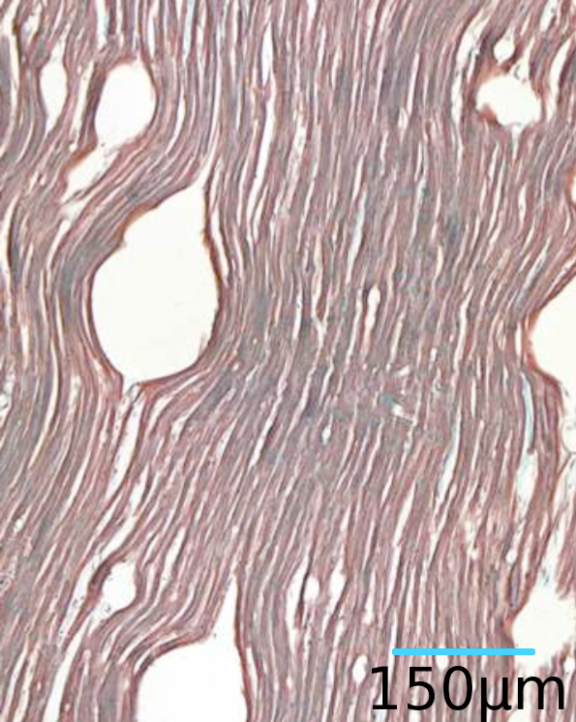
\includegraphics[height=55ex]{Ch4/Figs/histology}}
		\qquad
    \subfigure[][]{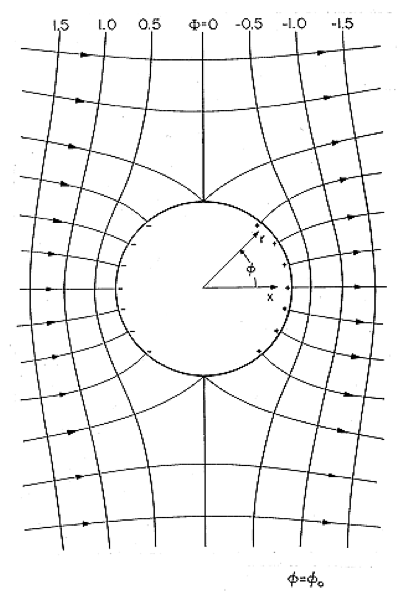
\includegraphics[height=55ex]{Ch4/Figs/cylinder}}
    \caption{\textbf{(a)} A 10$\mu$m-thick histological image of rabbit mid-myocardial wall long-axis slice, provided by \cite{Burton2006}. \textbf{(b)} The equipotentials (vertical lines) and field lines (horizontal with arrow heads) of a conducting circle in an infinite uniform field derived from the analytical solution to Eq. \ref{eqn:potential}.}
	  \label{fig:vessel}
	\end{figure}
  
  With the development of a more `accurate model' in mind, we note from the histological image in Figure~\ref{fig:vessel}(a) that muscle laminae are distorted by blood vessels and wrap around vasculature to accommodate it. A neat mathematical way to represent non-intersecting curved surfaces is to define a continuous scalar field over the domain of the volume, from here on referred to as a potential $\phi$, where the surfaces are the equipotentials of the field. Appealing to an electrostatic analogy, the solution to a conducting circle of radius $a$ in an infinite uniform field seems a helpful 2-dimensional starting point for a cylindrical vessel, and is depicted in Figure~\ref{fig:vessel}(b).
  
  We know that far away from the circle, the field is uniform and the potential is of the form
  
  \begin{equation}
    \Phi(r\rightarrow\infty) = -E_0y = -E_0r\cos\theta,
    \label{eqn:limit}
  \end{equation}
  
  where $E_0$ is the strength of the unperturbed uniform field. The potential produced by the charges on the edge of the circle must be added to this so that the edge is an equipotential,
  
  \begin{equation}
    \Phi(r=a) = 0.
    \label{eqn:condition}
  \end{equation}
  
  Any solution must satisfy Laplace's equation of zero divergence, as outside the circle
  
  \begin{equation}
    \nabla^2\Phi = \nabla\cdot\mathbf{E} = \frac{\rho}{\epsilon_0} = 0,
  \end{equation}
  
  where $\mathbf{E}$ is the electric field vector, $\rho$ is the volume charge density and $\epsilon_0$ is the permittivity of free space. It must also have the same $\theta$ dependence as equation~\ref{eqn:limit} and decay to zero at infinity, so that equation~\ref{eqn:limit} still holds. The solution takes the form
  
  \begin{equation}
    \Phi = \left(\frac{A}{r} - E_0r\right)\cos\theta,
  \end{equation}
  
  where $A$ is an arbitrary constant. Applying the boundary condition of equation~\ref{eqn:condition},
  
  \begin{equation}
    A = a^2E_0,
  \end{equation}
  
  the full expression for the potential becomes
  
  \begin{equation}
    \Phi = aE_0\left(\frac{a}{r} - \frac{r}{a} \right)\cos\theta\, .
    \label{eqn:potential}
  \end{equation}
  
  If $\theta$ is defined within the plane perpendicular to the vessel axis, this solution may be applied to any vessel whose axis lies within the $x$-$z$ plane, as is clear from Figure~\ref{fig:coplanar}.
  
  \begin{figure}[htbp]
    \centering
    \subfigure[][A vessel at zero potential in red, and an equipotential just below zero in blue.]{\label{fig:coplanar1}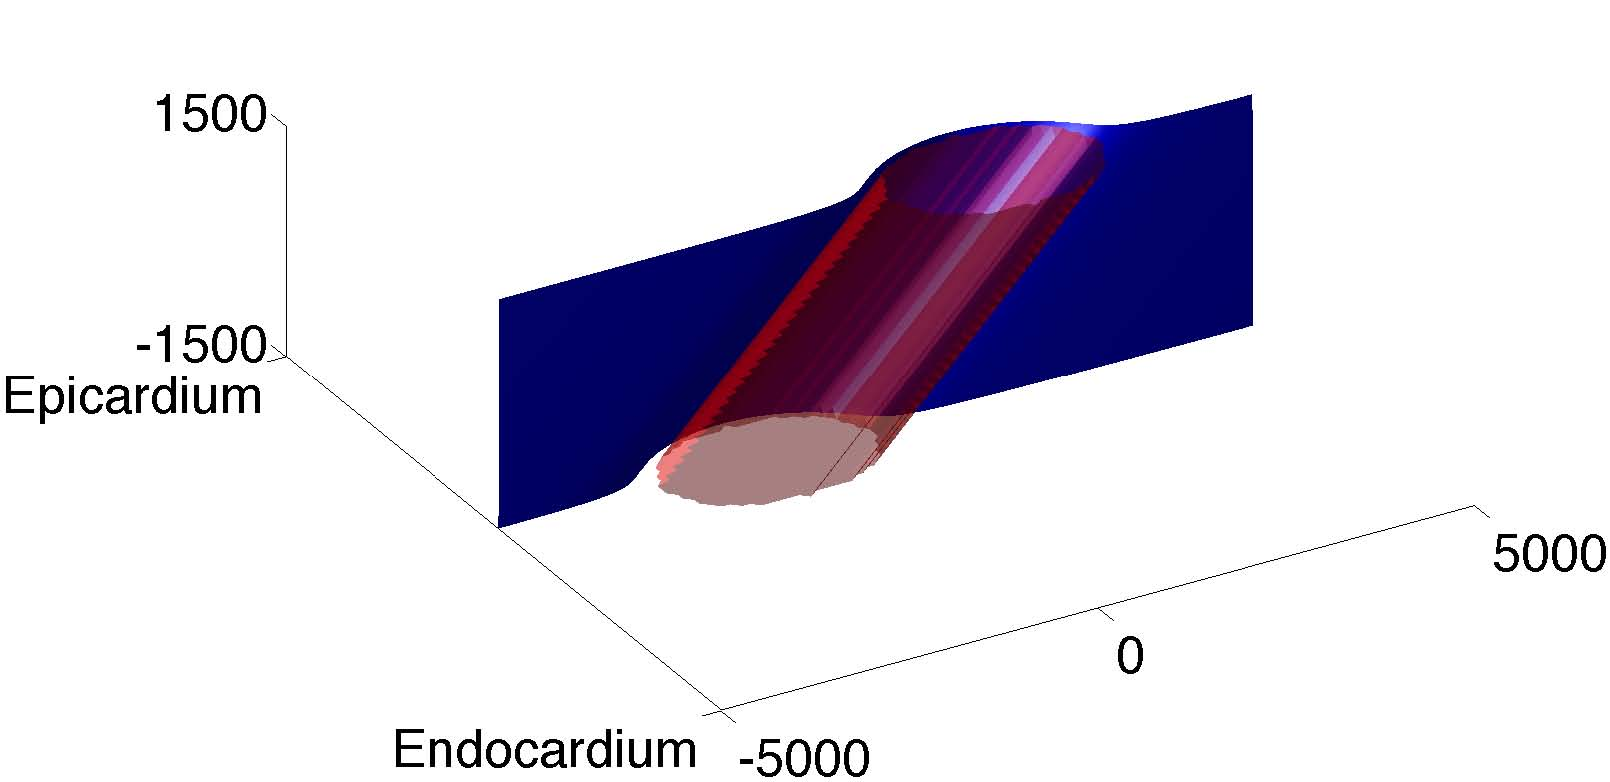
\includegraphics[width=0.7\textwidth]{Ch4/Figs/coplanar1}}
    \subfigure[][The same vessel with an equipotential just above zero.]{\label{fig:coplanar2}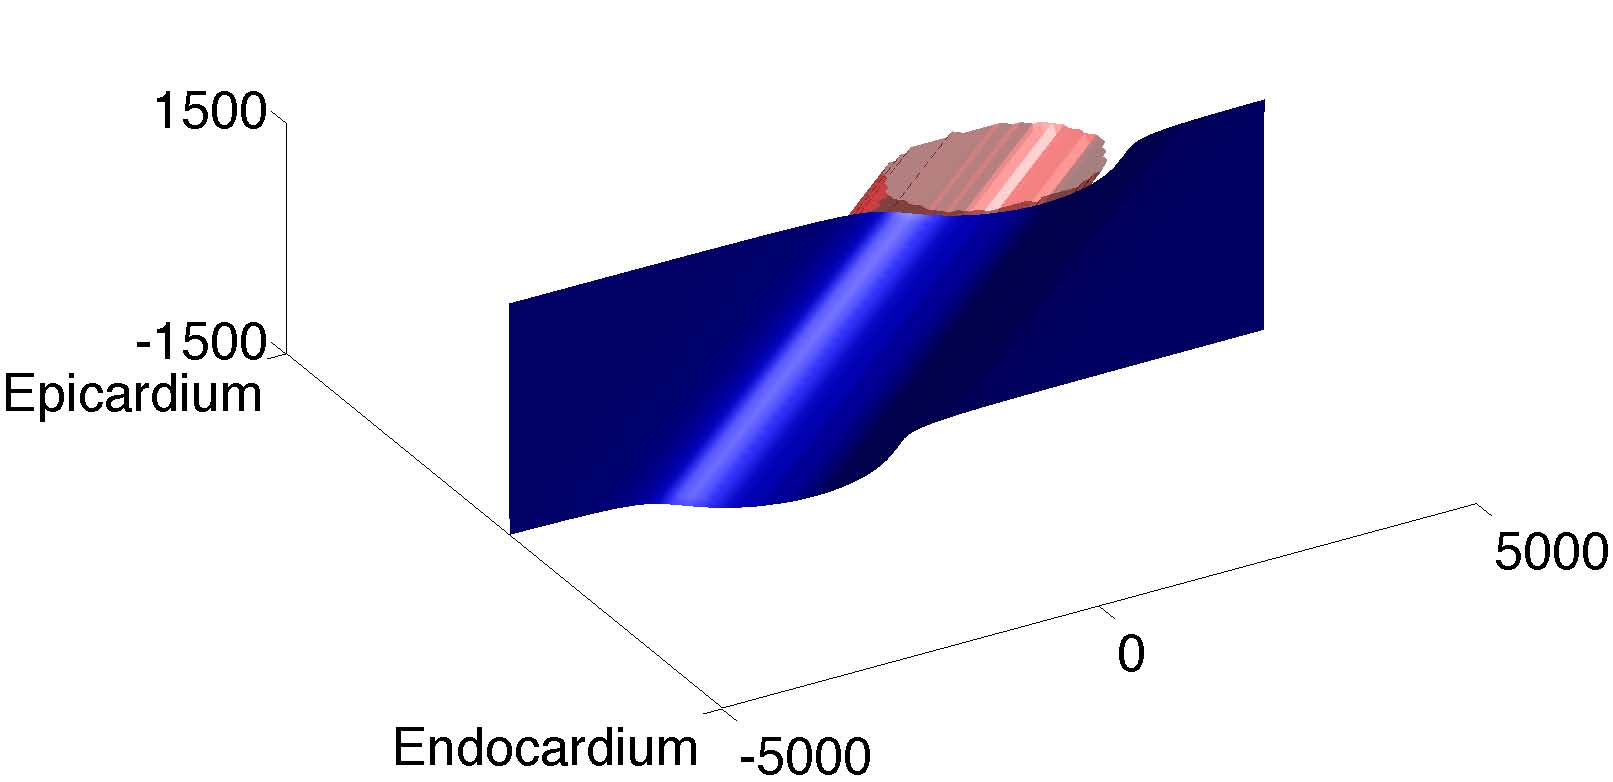
\includegraphics[width=0.7\textwidth]{Ch4/Figs/coplanar2}}
    \subfigure[][An equipotential further above zero.]{\label{fig:coplanar3}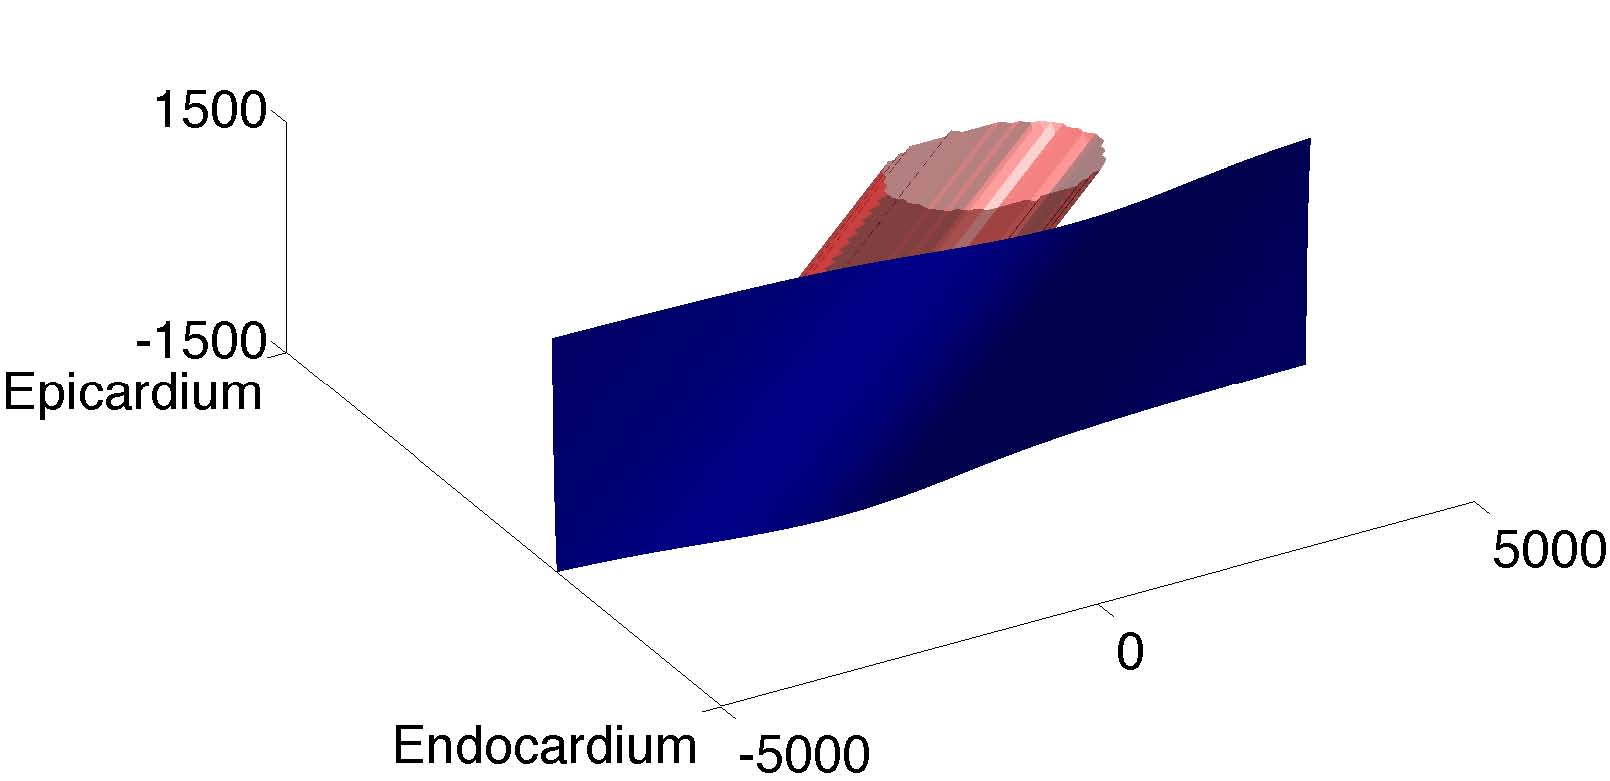
\includegraphics[width=0.7\textwidth]{Ch4/Figs/coplanar3}}
    \caption{A vessel lying parallel to the $x$-$z$ plane in red, and three different laminae (modelled as equipotentials) in blue, respectively. The first two pictures demonstrate the tight wrapping of the laminae around the vessel boundary, which is modelled as a conductor at zero potential, and thus is an equipotential itself. The third diagram illustrates how the deformation decreases with distance from the vessel. The vessel is pointing in the [1,0,1] direction.}
    \label{fig:coplanar}
  \end{figure}
  
  In the second regime, when the vessel is oriented along the $y$-direction, the model assumes that the tissue is displaced by the presence of the vessel only in the $x$- and $z$-directions. It is clear from Figure~\ref{fig:perpendicular} that the laminae are simply flat $x$-$z$ planes, just as they would be modelled in the absence of vasculature.
  
  \begin{figure}[htbp]
    \centering
    \subfigure[][Low $\Phi$.]{\label{fig:perpendicular1}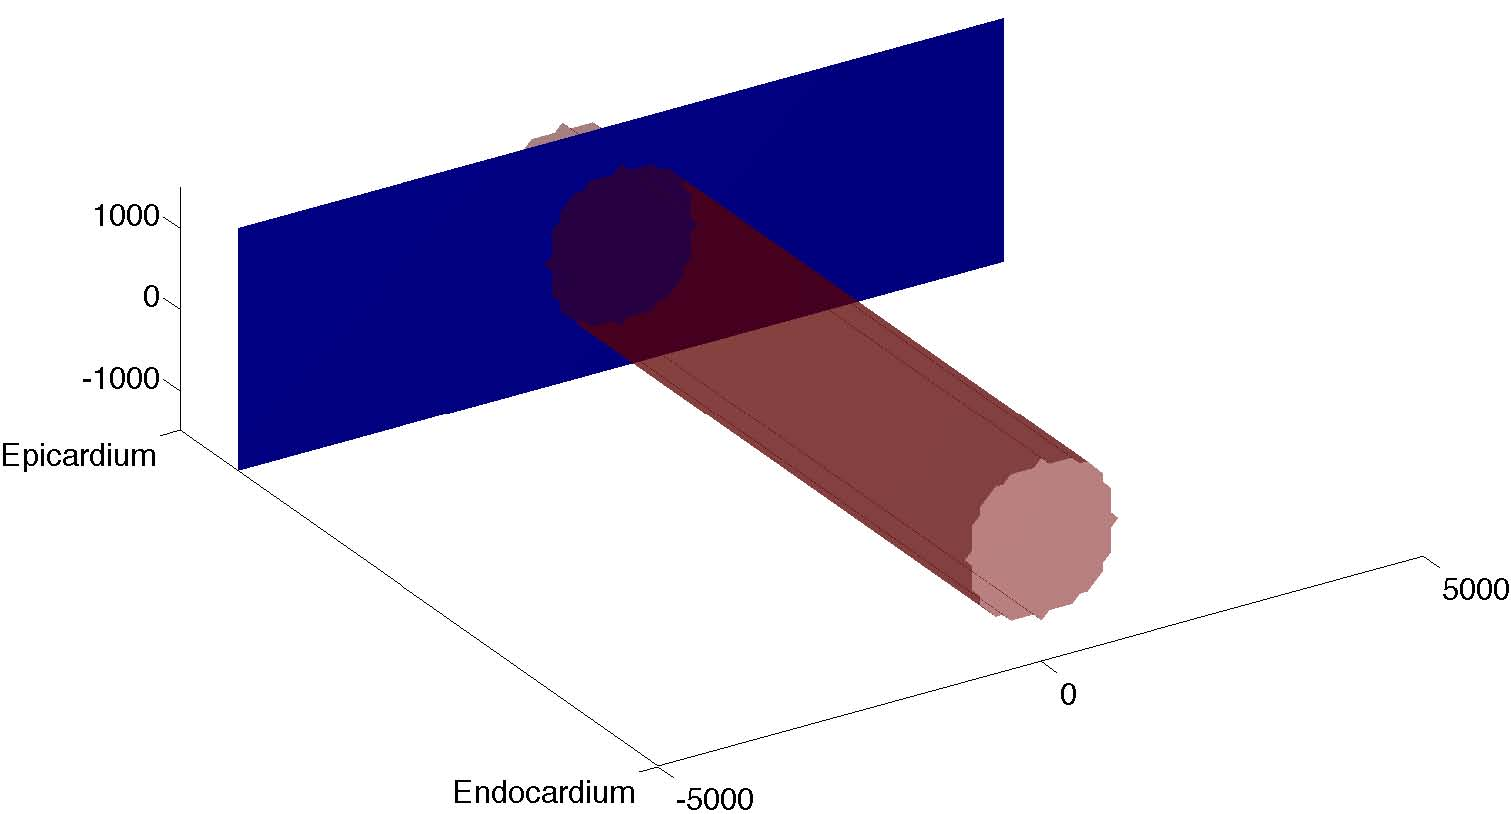
\includegraphics[width=0.7\textwidth]{Ch4/Figs/perpendicular1}}
    \subfigure[][Zero $\Phi$.]{\label{fig:perpendicular2}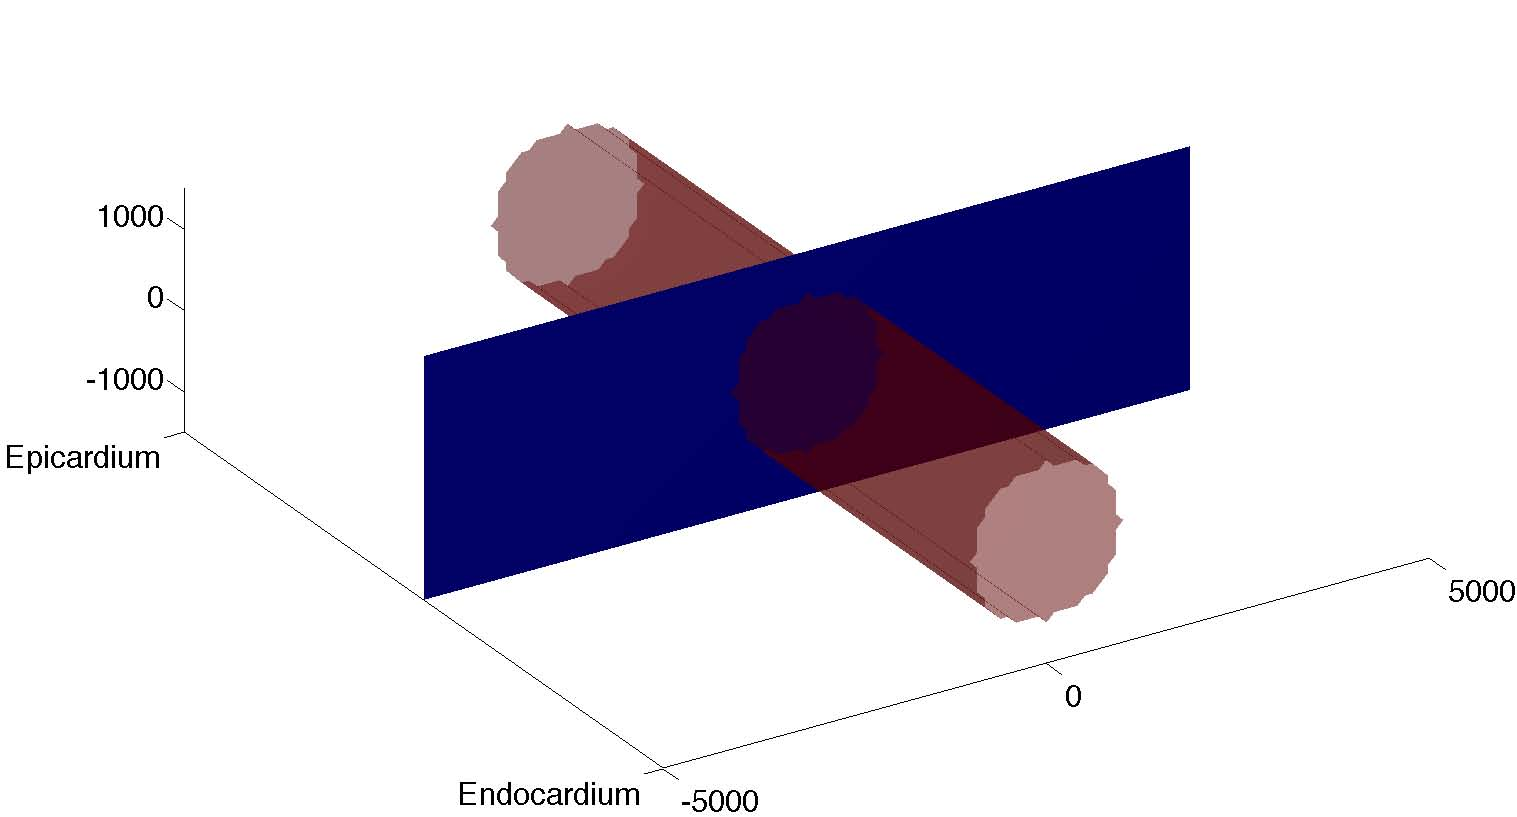
\includegraphics[width=0.7\textwidth]{Ch4/Figs/perpendicular2}}
    \subfigure[][High $\Phi$.]{\label{fig:perpendicular3}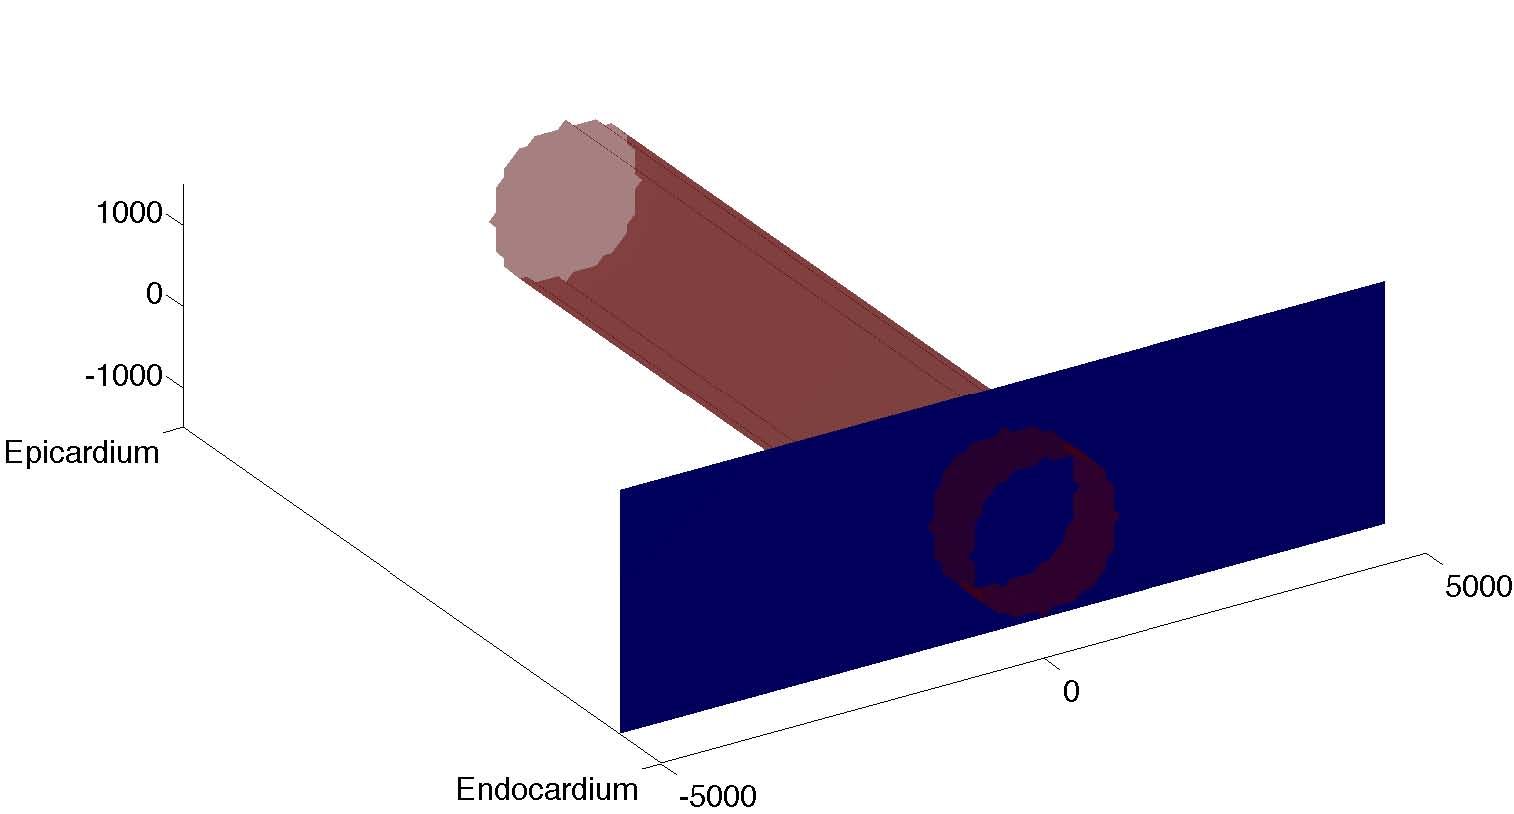
\includegraphics[width=0.7\textwidth]{Ch4/Figs/perpendicular3}}
    \caption{A vessel oriented along the $z$-axis, with three representative potential isosurfaces. It is assumed that a vessel perpendicular to the laminae only displaces the tissue in the $x$ and $z$ directions, thus the laminae remain in the same $x$-$z$ planes as if the vessel were not there. The blue isosurface is plotted inside the vessel boundary, but laminae are undefined within the vessel.}
    \label{fig:perpendicular}
  \end{figure}

  The third and final regime models a vessel that crosses laminae obliquely. How do the laminae deform and split around the vessel? In the absence of conclusive results through fibre registration at the time of modelling, the following assumption was made. Clearly, the laminae do not just deform in the $x$-$z$ plane, as in Figure~\ref{fig:perpendicular}. If they did, then a vessel pointing very slightly in the $y$-direction, e.g. [0, 0.01, 0], would carve an extremely long ellipse in each lamina.
  
  The approach taken here is a generalisation of the two cases in Figures~\ref{fig:coplanar} and Figures~\ref{fig:perpendicular}. The shortest distance from one side of a cylinder to the other is to move circularly around its radius, solely in the $\theta$ direction. The minimum cross-sectional area of a cylinder is observed when it is cut perpendicularly to its axis. Therefore, the minimum tear edge-length and hole area in a lamina that is split by a blood vessel occurs when the lamina wraps the vessel on a circular cross-section. This is how the vessel-lamina interface was modelled and the results can be seen in Figure~\ref{fig:oblique}. The following paragraphs are a mathematical discussion of the way this constraint was implemented. First we must define a point in the tissue in vascular coordinates.
  
  \begin{figure}[htbp]
    \centering
    \subfigure[][Low $\Phi$.]{\label{fig:oblique_no_vessel1}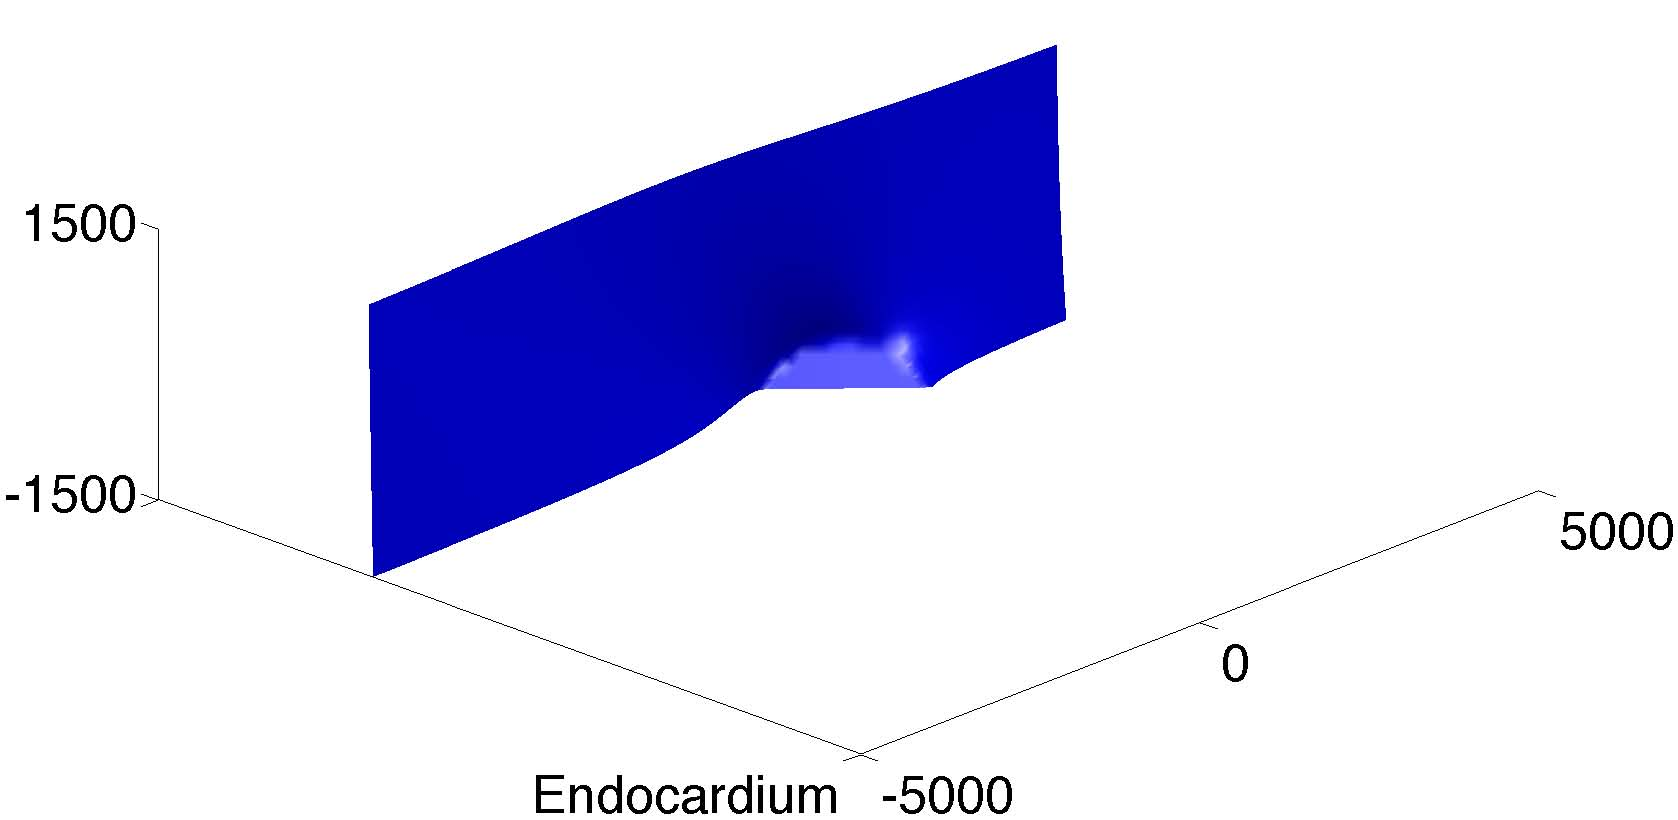
\includegraphics[width=0.469\textwidth]{Ch4/Figs/oblique_no_vessel1}} \qquad
    \subfigure[][Low $\Phi$ with rendered vessel.]{\label{fig:oblique_vessel1}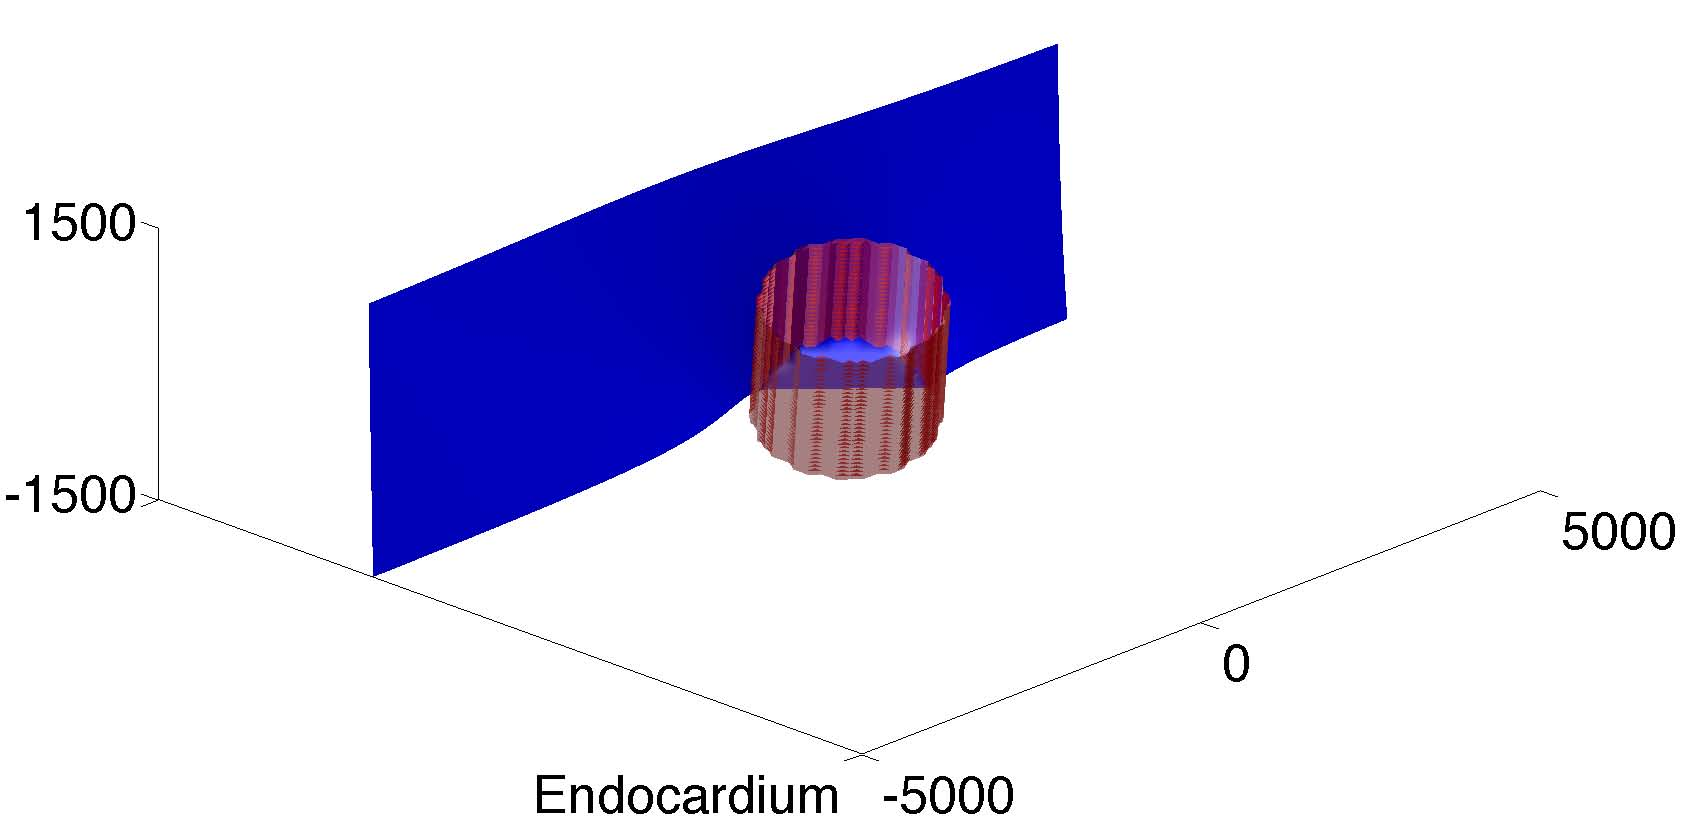
\includegraphics[width=0.469\textwidth]{Ch4/Figs/oblique_vessel1}}
    \subfigure[][Zero $\Phi$.]{\label{fig:oblique_no_vessel2}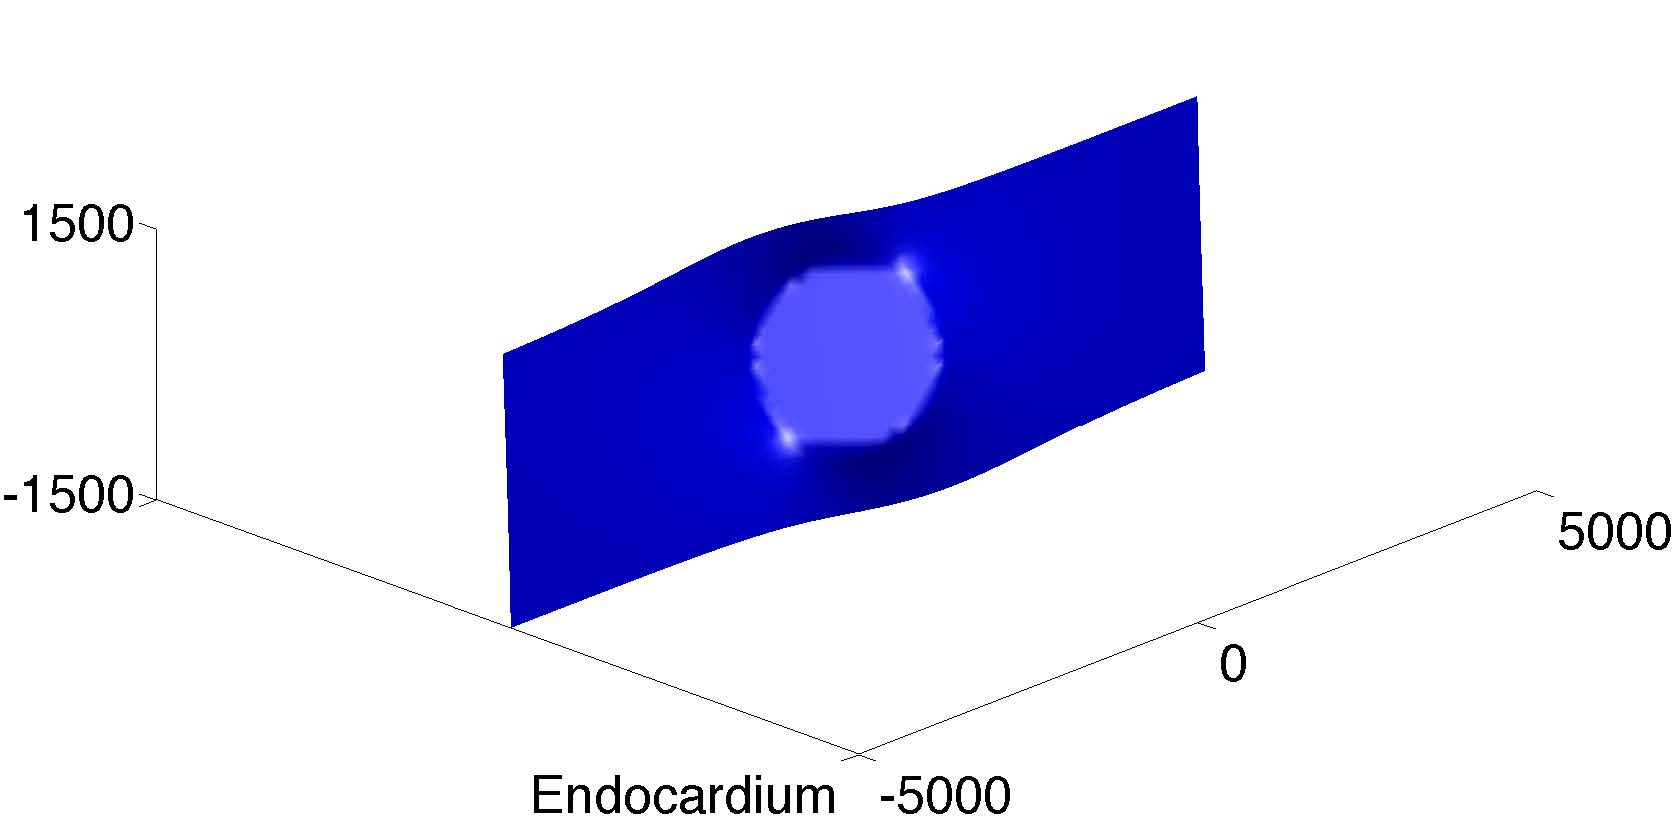
\includegraphics[width=0.469\textwidth]{Ch4/Figs/oblique_no_vessel2}} \qquad
    \subfigure[][Zero $\Phi$ with rendered vessel.]{\label{fig:oblique_vessel2}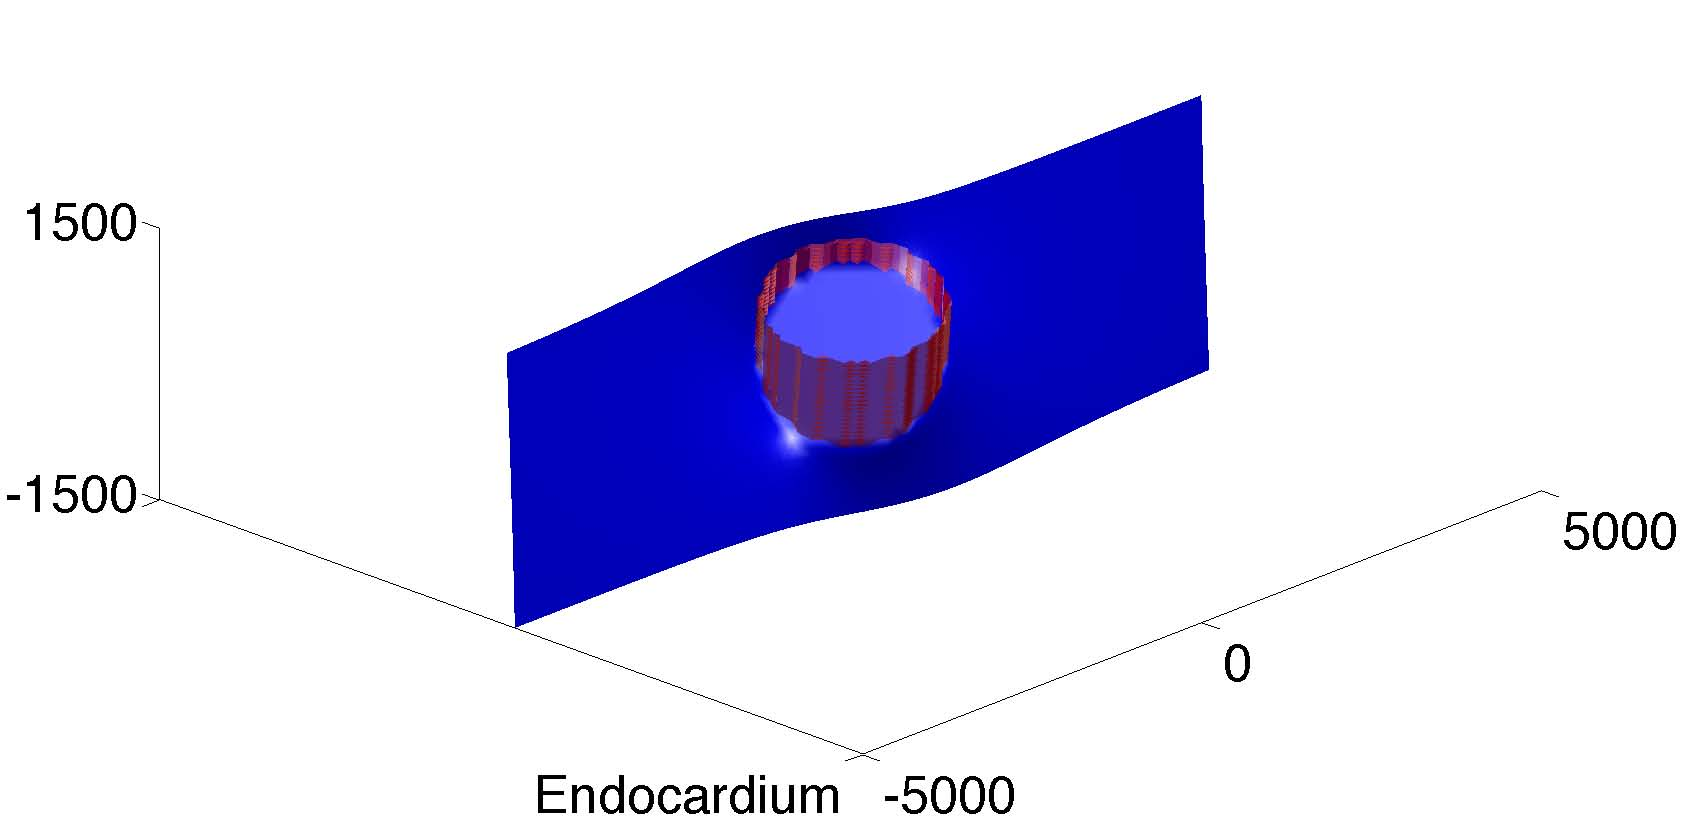
\includegraphics[width=0.469\textwidth]{Ch4/Figs/oblique_vessel2}}
    \subfigure[][High $\Phi$.]{\label{fig:oblique_no_vessel3}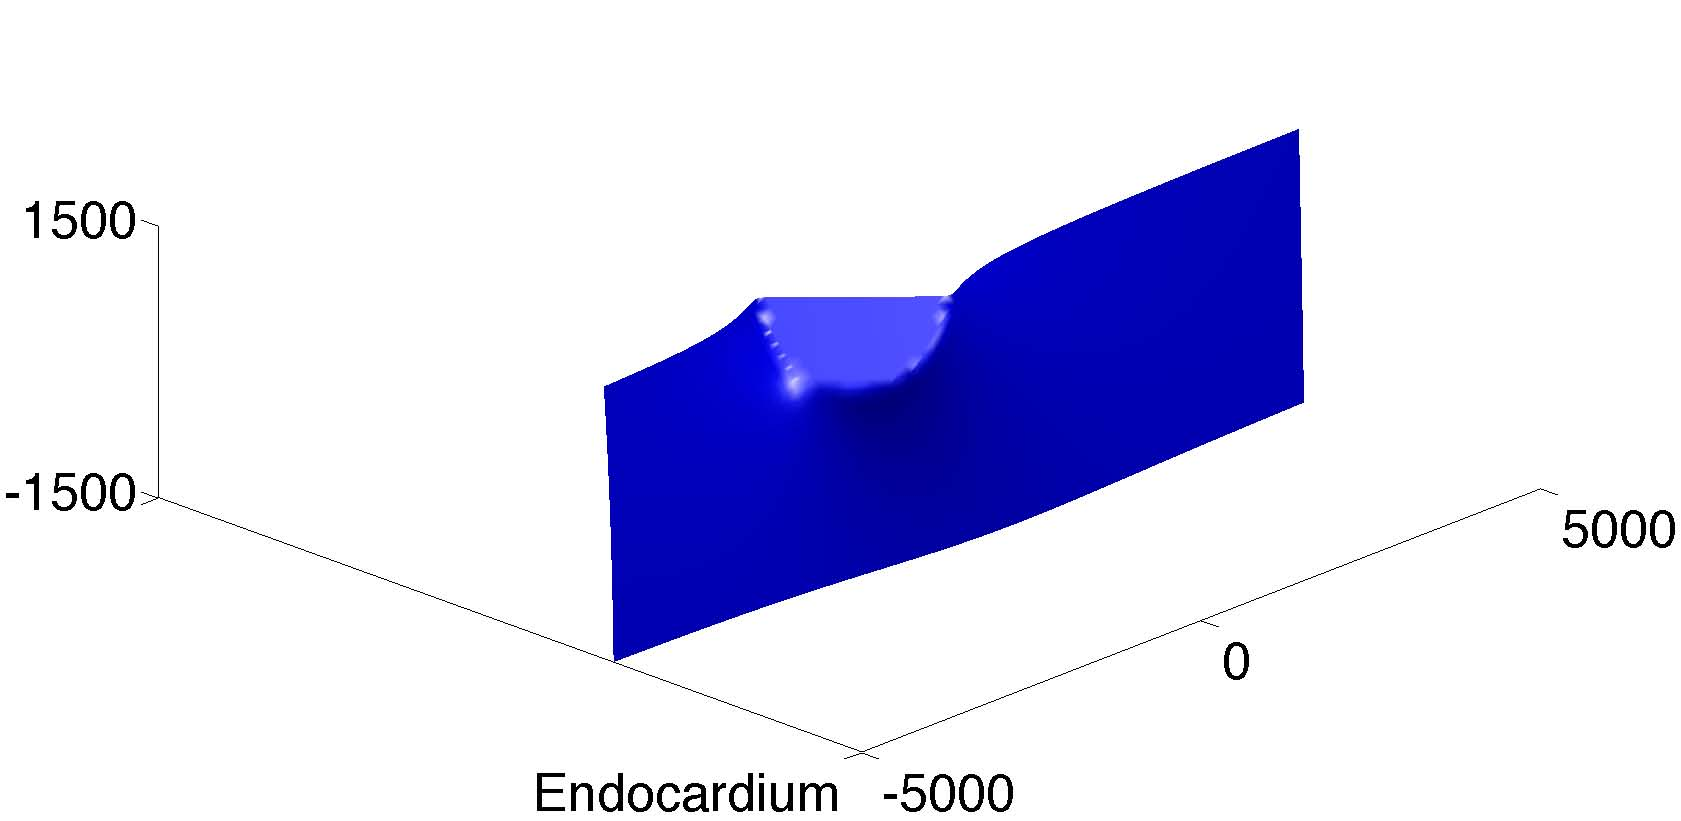
\includegraphics[width=0.469\textwidth]{Ch4/Figs/oblique_no_vessel3}} \qquad
    \subfigure[][High $\Phi$ with rendered vessel.]{\label{fig:oblique_vessel3}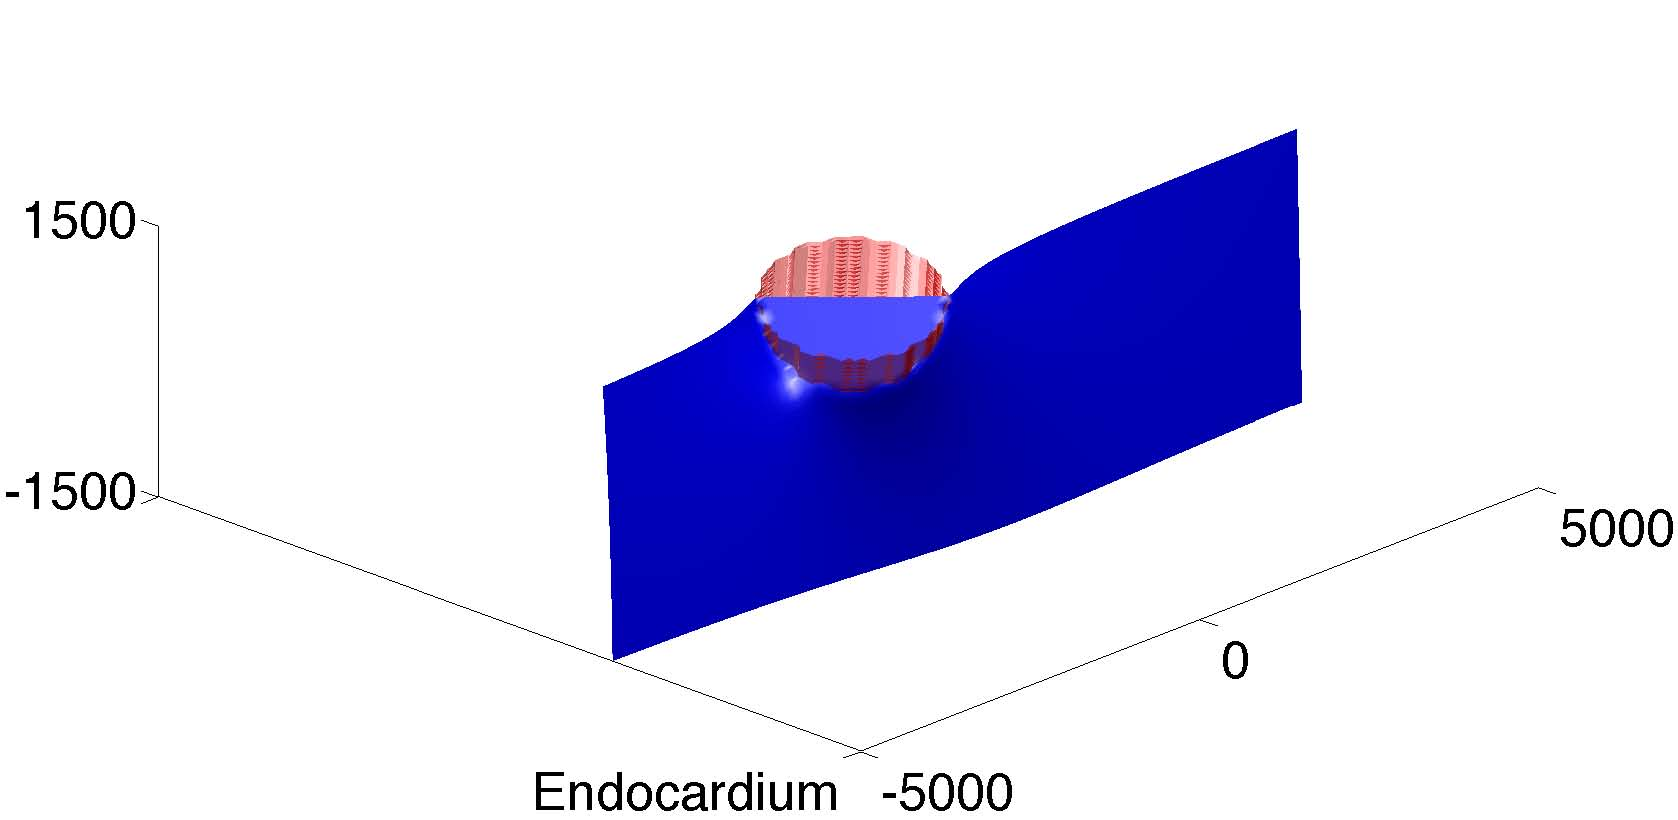
\includegraphics[width=0.469\textwidth]{Ch4/Figs/oblique_vessel3}}
    \caption{An oblique vessel is modelled, oriented in the direction [1,1,-1]. In order to show clearly the laminae (surfaces of equal $\Phi$) close to the vessel boundary, each lamina is plotted with and without the vessel being rendered. Again, despite the illuminated circle of the blue surfaces being plotted, the laminae are undefined within the vessel.}
    \label{fig:oblique}
  \end{figure}
  
  To calculate the potential at any given point \textbf{x}, its coordinates are first represented in the cylindrical coordinate system of the vessel, so that $\mathbf{x} = \mathbf{x}(r,\theta,h)$. When $\theta = 0$, the unit vector in the $r$-direction $\mathbf{e}_r$ is defined as
  
  \begin{equation}
    \mathbf{e}_r(\theta = 0) =  \mathbf{e}_{r0} = \frac{\mathbf{e}_y - (\mathbf{e}_h \cdot \mathbf{e}_y) \mathbf{e}_h}{\sqrt{1 - \left(\mathbf{e}_h \cdot \mathbf{e}_y\right)^2}},
  \end{equation}
  
  or, put another way, the normalised component of $\mathbf{e}_y$ perpendicular to $\mathbf{e}_h$. Far away from the vessel, the field points in the direction of -$\mathbf{e}_y$ and so the potential increases along $\mathbf{e}_y$. Thus this is the direction in a cross-sectional plane of the steepest mean potential gradient.
  
  Having defined the cylindrical coordinate system, the tissue potential must be expressed as a function of these coordinates. The total potential can be considered as the sum of two components, that due to its $h$-coordinate, and that due to its position in the plane of that $h$-coordinate:
  
  \begin{equation}
    \Phi = \Phi_{\text{axis}} + \Phi_{\text{plane}}\,.
  \end{equation}
  
  Since we wish the laminae to deform symmetrically around the vessel, it makes sense to set the potential along the axis, $\mathbf{x}(0,0,h)$, to what it would have been in the absence of a vessel. From equation \ref{eqn:limit},
  
  \begin{align}
    \Phi_{\text{axis}} & = -E_0h(\mathbf{e}_h \cdot \mathbf{e}_y) \\
    & = -E_0h\cos\phi,
  \end{align}
  
  where $\phi$ is the angle between the y-axis and the vessel axis. The planar potential can then be described by the 2D solution \ref{eqn:potential} (graphically displayed in Figure~\ref{fig:vessels}(b)), with a factor to account for the angle between the plane and the uniform field direction $\mathbf{e}_y$:
  
  \begin{align}
    \Phi_{\text{plane}} &= -aE_0\left( \frac{r}{a} - \frac{a}{r} \right) \cos \theta \left(\mathbf{e}_{r0} \cdot \mathbf{e}_y \right) \\
    &= -aE_0\left( \frac{r}{a} - \frac{a}{r} \right) \cos \theta \sqrt{ 1 - \left( \mathbf{e}_h \cdot \mathbf{e}_y \right)^2 } \\
    &= -aE_0\left( \frac{r}{a} - \frac{a}{r} \right) \cos \theta \sin \phi \, .
  \end{align}
  
  We can now describe the potential at any point in the tissue,
  
  \begin{equation}
    \Phi = -E_0\left[ h \cos \phi + a \left( \frac{r}{a} - \frac{a}{r} \right) \cos \theta \sin \phi \, \right].
    \label{eqn:potential_3D}
  \end{equation}
  

\subsection{Defining the Fibre Direction Within the Laminae}
\label{sec:defining_the_fibre_direction_within_the_laminae}
  Having defined the myocardial laminae, a fibre direction must be modelled within them. This modelling consists of 3 stages:
  
  \begin{itemize}
    \item calculating $\nabla\Phi$,
    \item projecting a compressed form of the 2D solution \ref{eqn:potential} along $\mathbf{e}_y$ onto each lamina,
    \item normalising the cross-product of these two vectors.
  \end{itemize}
  
  \subsubsection{Calculating $\nabla\Phi$}
  \label{sub:calculating_nablaphi}
    Fibres must always lie within the lamina surface and are therefore perpendicular to the potential gradient. This gradient can be obtained simply as the spatial differential of equation~\ref{eqn:potential_3D}; the results are visualised in Figure~\ref{fig:del_phi}.
    
    \begin{figure}[htbp]
      \centering
      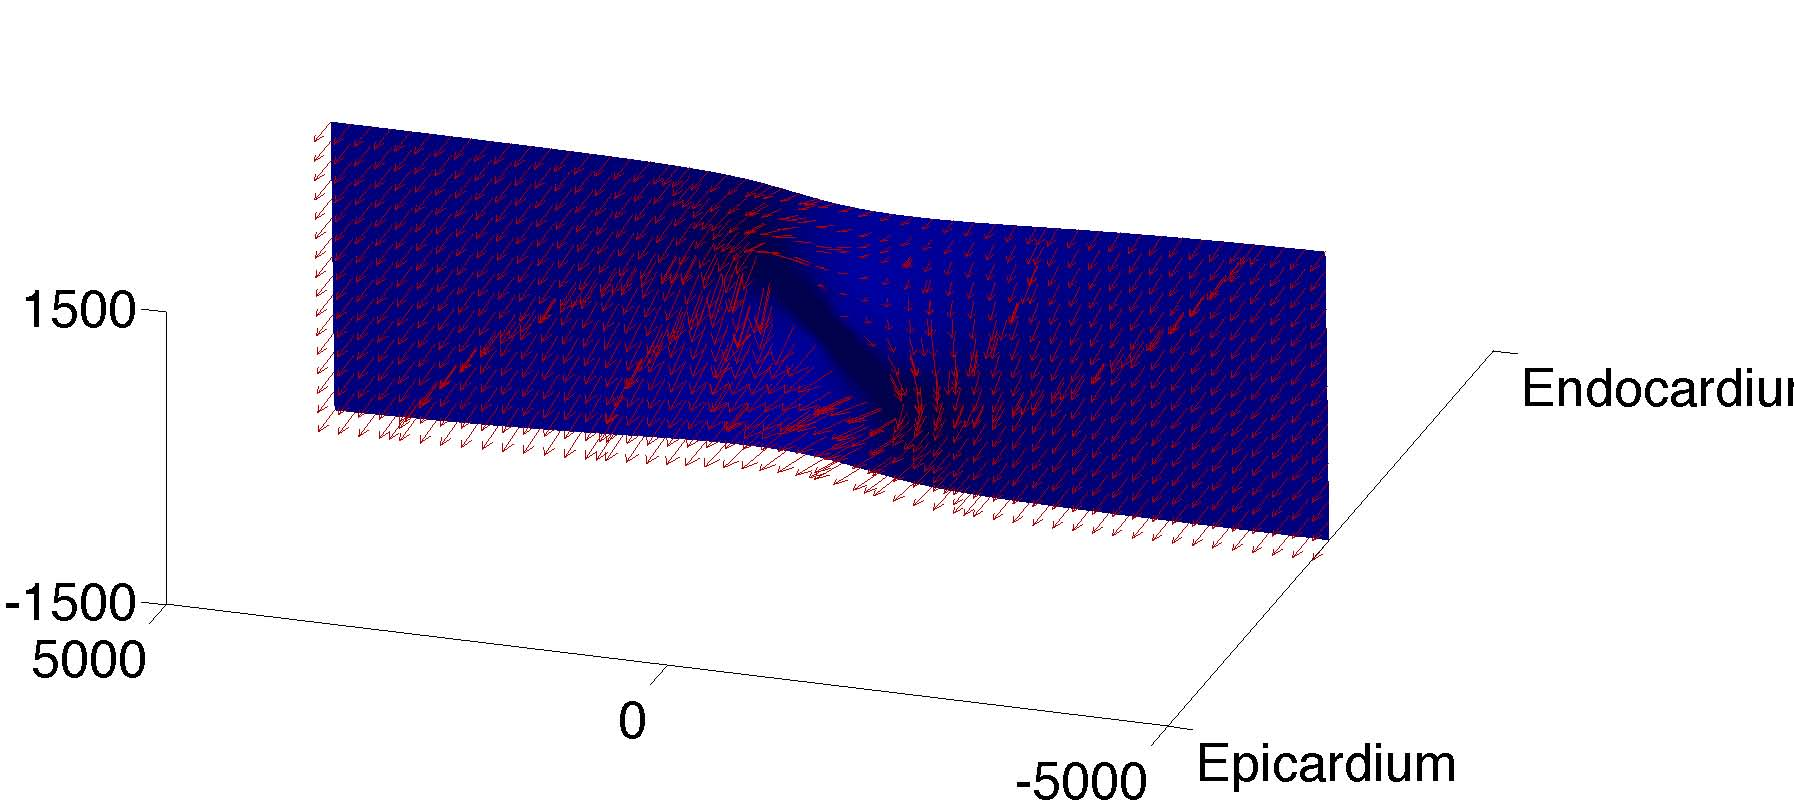
\includegraphics[width=1\textwidth]{Ch4/Figs/del_phi}
      \caption{A 3D quiver plot of $\nabla\Phi$ at an array of points on an equipotential.}
      \label{fig:del_phi}
    \end{figure}
  
  \subsubsection{Projecting a 2D Solution} % (fold)
  \label{sub:projecting_a_2_d_solution}
    When viewed along the $y$-axis, the circular sheet boundary describes an ellipse, with semimajor radius equal to the vessel radius and semiminor radius shorter by a factor of $\cos \phi$. The isolines of equation~\ref{eqn:potential} in Figure~\ref{fig:vessel}(b) can be compressed by $\cos \phi$ and mapped onto a lamina, so that the isolines at the edge of the ellipse are tangent to it. A grid of vectors perpendicular to these isolines is shown in Figure~\ref{fig:projected}. From here on, we shall refer to the 2D coordinate system $\left[ x, y \right]$ in the tissue coordinates as compressed, and the system $\left[ x', y' \right]$ in the natural coordinates of equation~\ref{eqn:potential} as non-compressed.
    
    \begin{figure}[htbp]
      \centering
      \subfigure[][A view along the $x$-axis, showing the vessel intersecting the surface.]{\label{fig:projected1}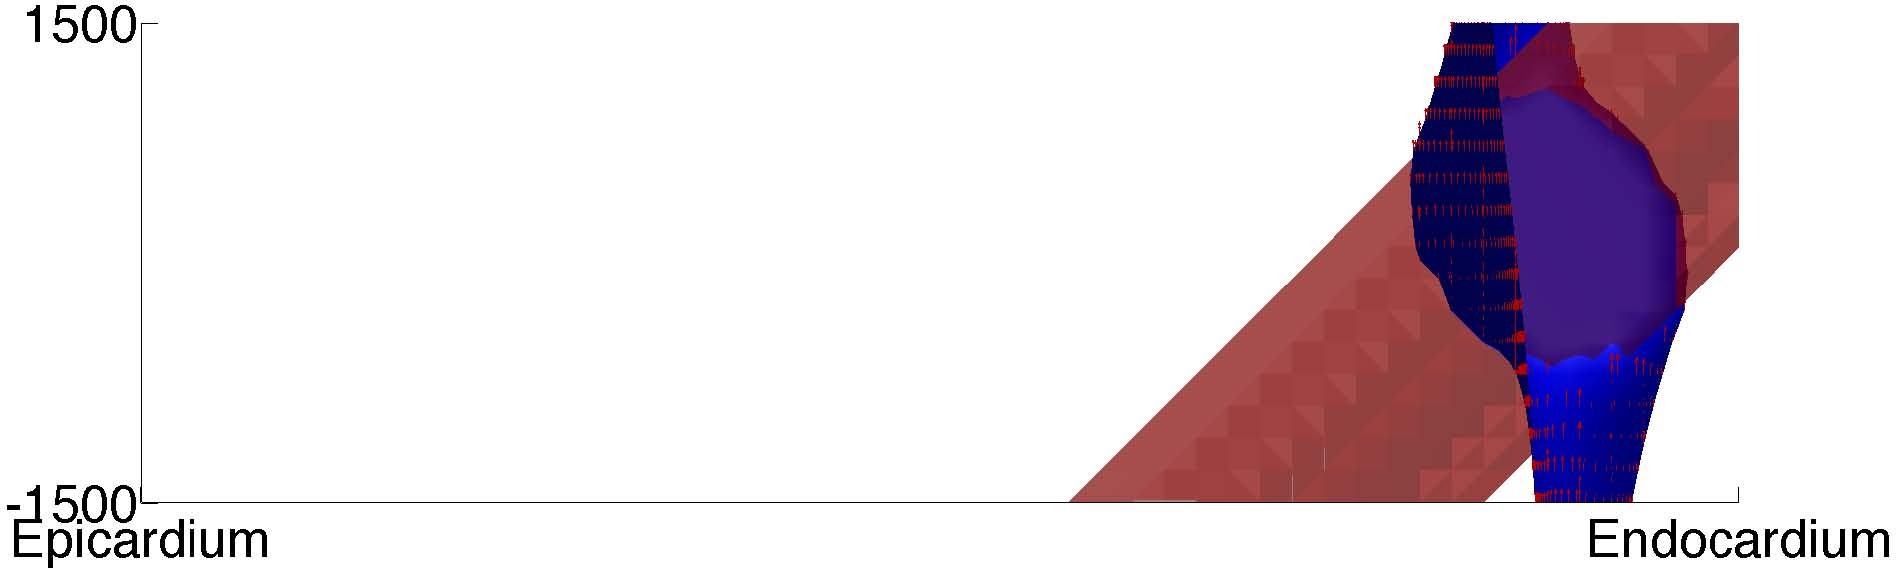
\includegraphics[width=1\textwidth]{Ch4/Figs/projected1}}
      \subfigure[][The same view, with no vessel rendering and translucent surface rendering. The quivers are more visible and it is clear that none have a $y$-component.]{\label{fig:projected2}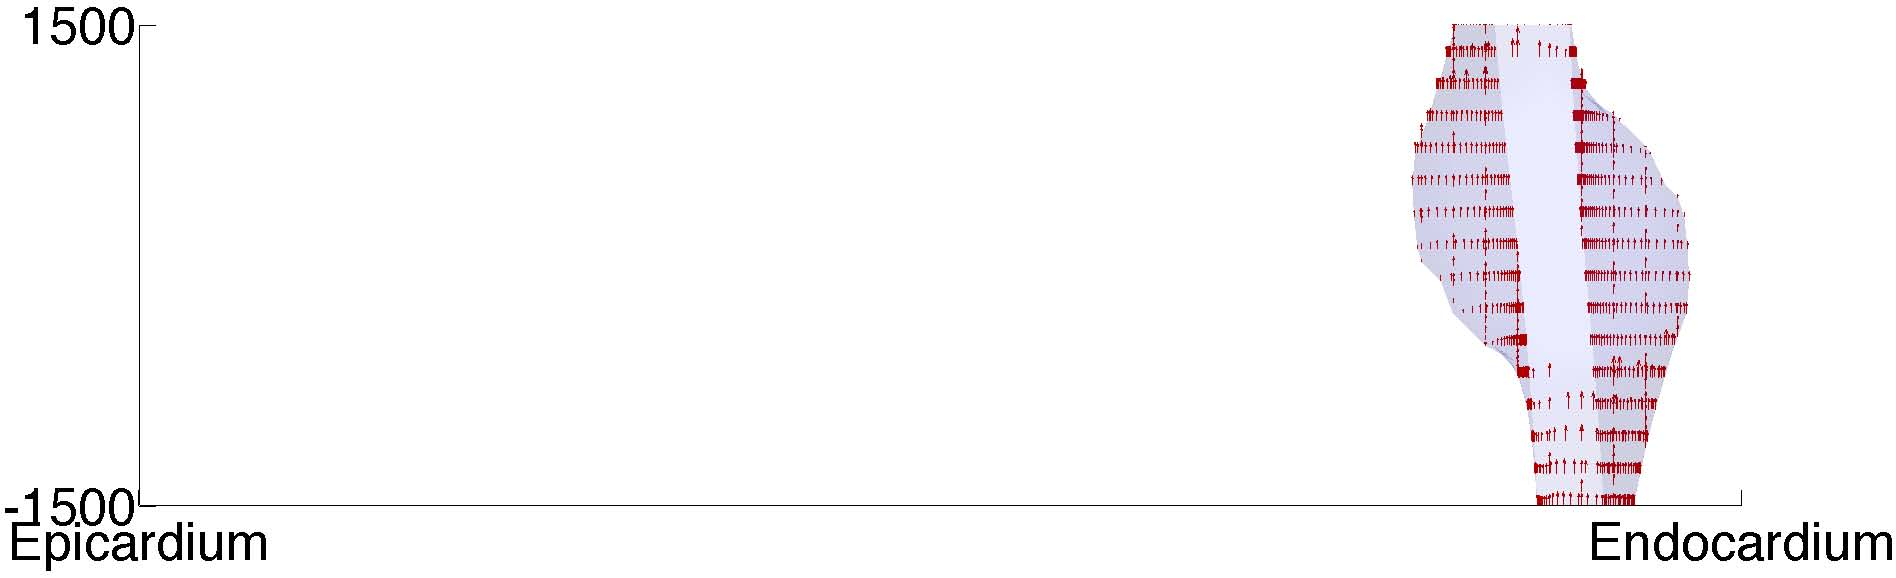
\includegraphics[width=1\textwidth]{Ch4/Figs/projected2}}
      \subfigure[][A view along the $y$-axis. The vectors in the $x$-$z$ plane have a direction trend up and to the left, at $90^\circ$ to $\alpha$. However, at the edge of the ellipse, where the vessel intersects the lamina, all vectors are perpendicular to the elliptical projection of the circle onto the $x$-$z$ plane.]{\label{fig:projected3}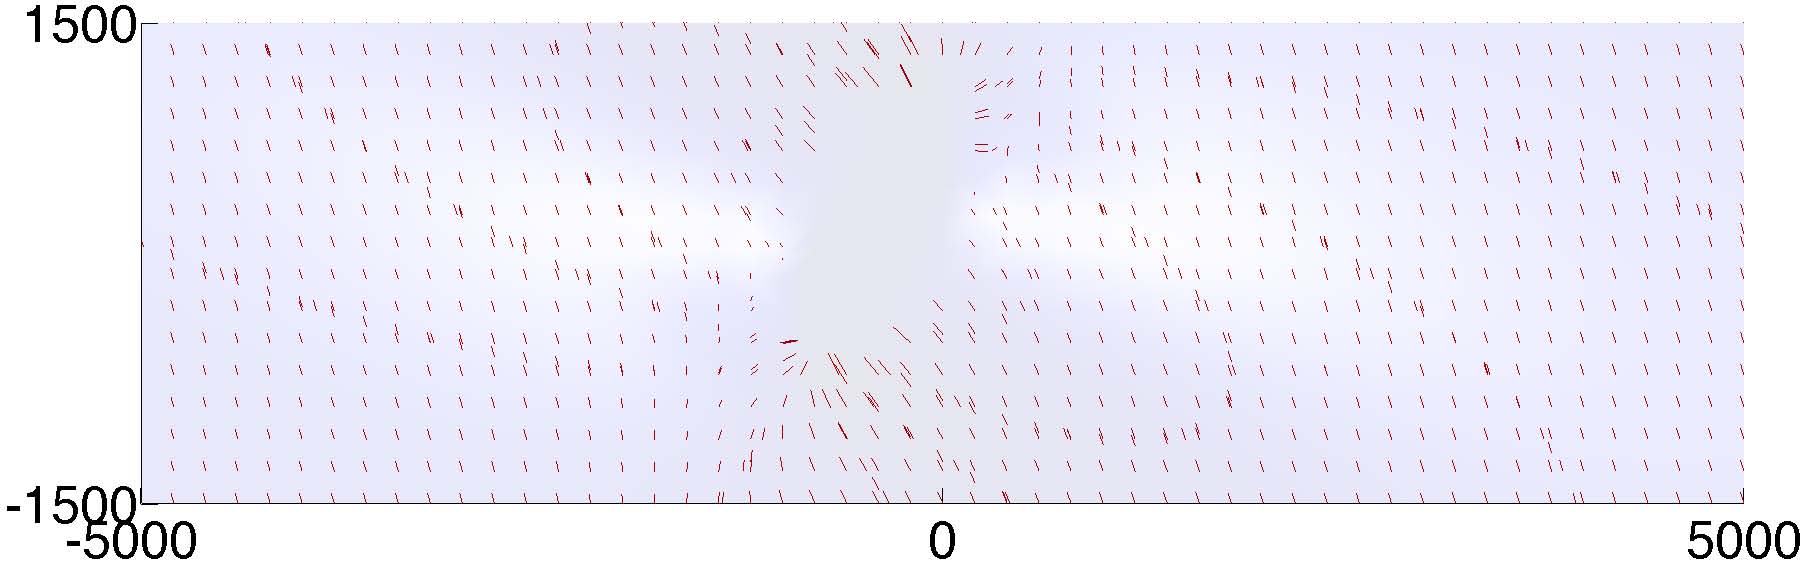
\includegraphics[width=1\textwidth]{Ch4/Figs/projected3}}
      \caption{A 3D quiver plot of the compressed 2D solution, plotted on the same isosurface as in Figures~\ref{fig:oblique_vessel} and \ref{fig:oblique_no_vessel}.}
      \label{fig:projected}
    \end{figure}

    The questions remains, in which orientation should solution~\ref{eqn:potential} be mapped? The following cubic dependency of overall fibre direction on depth of myocardial tissue has been observed experimentally \cite{Potse2006,StreeterJr1969}. Let $e$ be a tissue depth parameter

    \begin{equation}
      e = \frac{\Phi_\text{endo}}{\Phi_\text{endo}+\Phi_\text{epi}}\,,
    \end{equation}

    where $\Phi_\text{endo}$ and $\Phi_\text{epi}$ are the potentials at the endocardium and epicardium, respectively. Then the fibre angle from the horizontal $\alpha$, graphed in Figure~\ref{fig:transmural_variation}, is modelled to vary transmurally such that

    \begin{equation}
      \alpha = \frac{\pi}{3} \left( 1 - 2e \right)^3\,.
    \end{equation}
    
    \begin{figure}[htbp]
      \centering
      \subfigure[][Depth parameter $e$ against $\alpha$.]{\label{fig:transmural_variation1}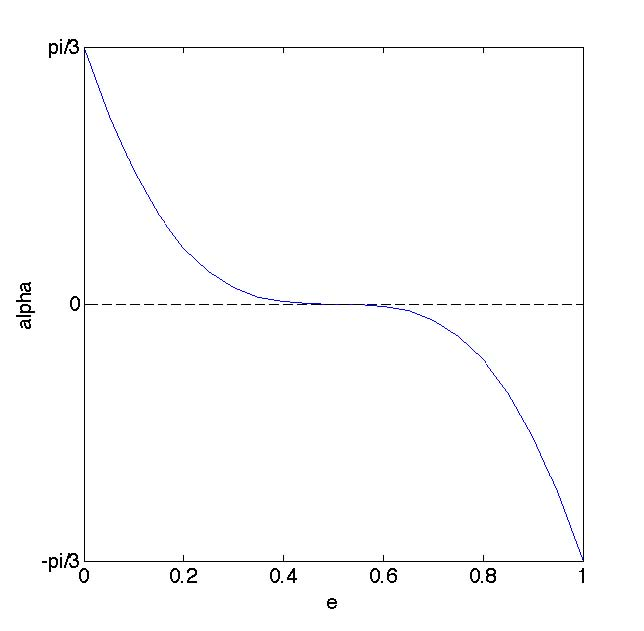
\includegraphics[width=0.469\textwidth]{Ch4/Figs/transmural_variation1}} \qquad
      \subfigure[][Depth parameter $e$ against unit direction vectors plotted in the x-z plane.]{\label{fig:transmural_variation2}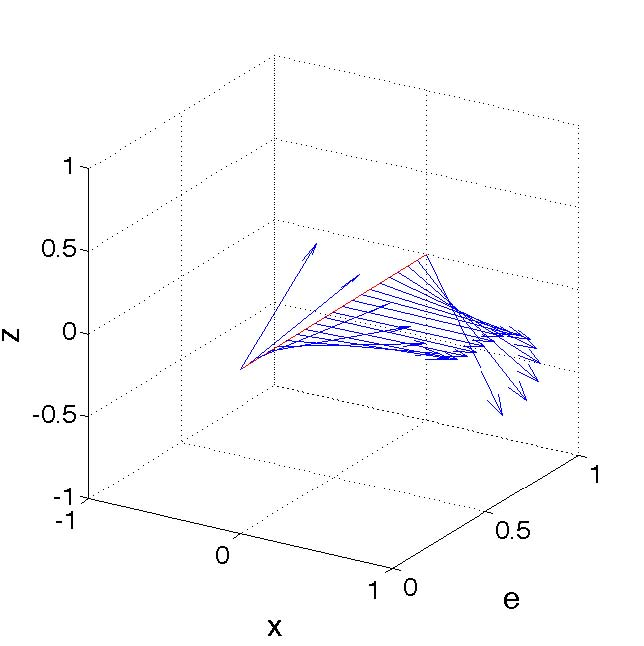
\includegraphics[width=0.469\textwidth]{Ch4/Figs/transmural_variation2}}
      \caption{Two representations of the transmural variation in $\alpha$.}
      \label{fig:transmural_variation}
    \end{figure}

    Let $u(x,z)$ and $v(x,z)$ be the components of a unit vector in the x-z plane at an angle $\alpha$ from the x-axis
    
    \begin{equation}
      \left( \begin{array}{c}
        u \\
        v
      \end{array} \right)
       =
       \left( \begin{array}{c}
         \cos \alpha \\
         \sin \alpha
       \end{array} \right)\,.
    \end{equation}
    
    Then the components in the non-compressed coordinates $u'\left(x',z'\right)$ and $v'\left(x',z'\right)$ are found by applying three transformations. First the axes are rotated through the angle $\gamma$, between the projection of the vessel orientation onto the $x$-$z$ plane and the $x$-axis. This rotation aligns the semiminor axis of the ellipse with the $x$-axis and the semimajor with the $y$-axis. Then the ellipse is stretched along the x-axis to become circular, and finally the inverse rotation is applied to the result:
    
    \begin{equation}
      \left( \begin{array}{c}
        u' \\
        v'
      \end{array} \right)
      =
      \left( \begin{array}{cc}
        \cos \gamma & - \sin \gamma \\
        \sin \gamma &   \cos \gamma
      \end{array} \right)
      \left( \begin{array}{cc}
        1/\cos \phi & 0 \\
        0 & 1
      \end{array} \right)
      \left( \begin{array}{cc}
         \cos \gamma & \sin \gamma \\
        -\sin \gamma & \cos \gamma
      \end{array} \right)
      \left( \begin{array}{c}
        u' \\
        v'
      \end{array} \right) .
    \end{equation}
    
    The mean fibre angle from the horizontal in the non-compressed frame is therefore
    
    \begin{equation}
      \alpha' = \arctan \frac{u'}{v'}\,.
    \end{equation}
    
    This angle must be added at all points on the lamina as a constant rotation of the solution~\ref{eqn:potential}, so that in the non-compressed coordinate system
    
    \begin{equation}
      \Psi(r',\theta') = -aE_0 \left( \frac{r}{a} - \frac{a}{r} \right) \cos\left( \theta' + \alpha' \right)\,,
      \label{eqn:potential_projected}
    \end{equation}
    
    where $r'$ and $\theta'$ are the non-compressed 2D polar coordinates.
  
  \subsubsection{Normalising the Cross Product} % (fold)
  \label{sub:normalising_the_cross_product}
    The final stage in defining fibre direction is to calculate $\chi$ the normalised cross-product of the results from the previous two sections: 
    \begin{equation}
      \chi = \frac{\nabla\Phi \times \nabla\Psi}{\lvert\nabla\Phi \times \nabla\Psi\rvert},
    \end{equation}
      where $\nabla\Phi$ is the 3D gradient of equation~\ref{eqn:potential_3D} and $\nabla\Psi$ is the 3D vector constructed from the 2D gradient of equation~\ref{eqn:potential_projected} in the $x$- and $z$-directions and zero in the $y$-direction. At any point in the tissue, the resulting fibre vector will lie tangential to the lamina. A vector will also lie tangential to the vessel boundary, should it reside there. Figures~\ref{fig:oblique_vessel} and \ref{fig:oblique_no_vessel} display the final results from three different viewpoints.
    
    \begin{figure}[htbp]
      \centering
      \vspace{-2.5em}
      \subfigure[][]{\label{fig:oblique_vessel1}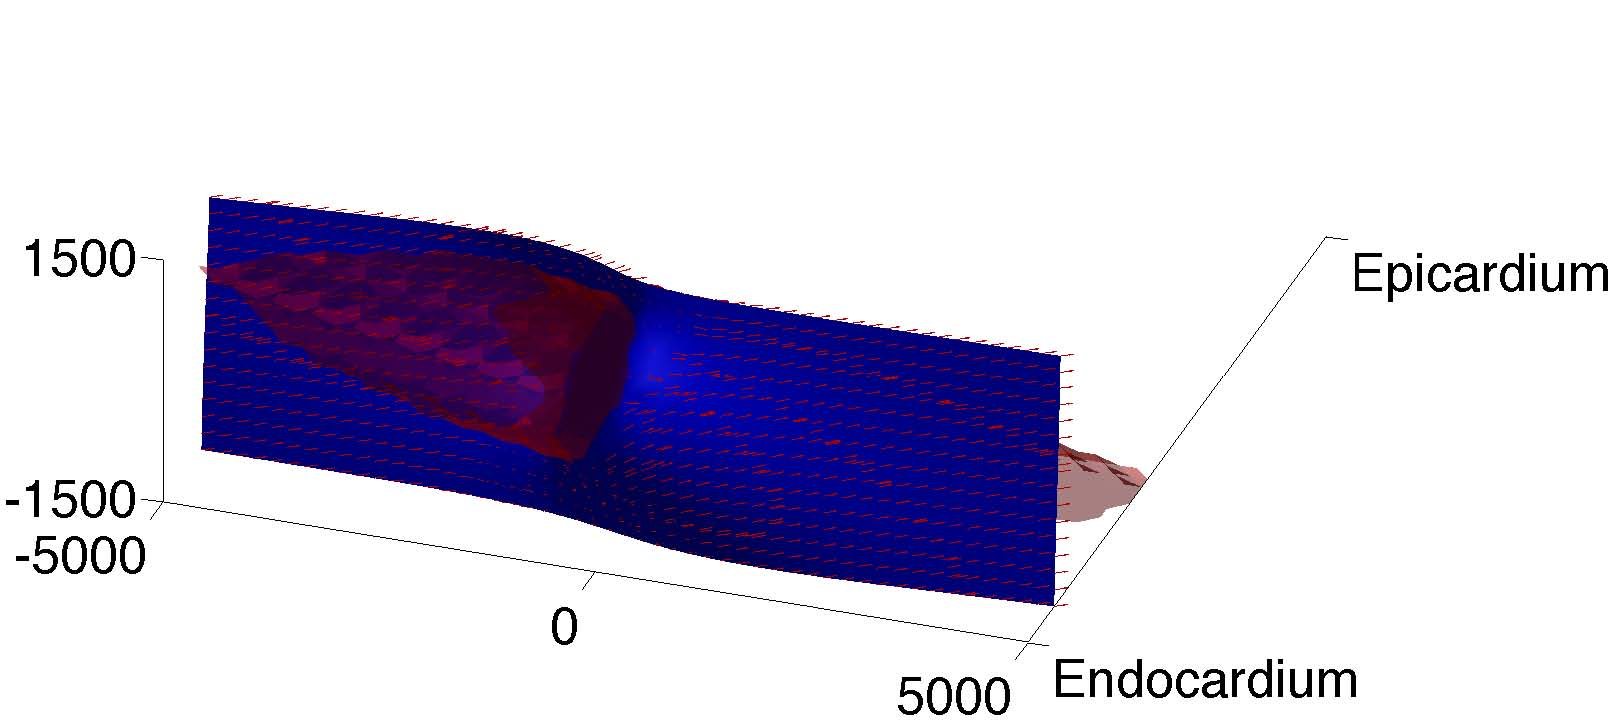
\includegraphics[width=1\textwidth]{Ch4/Figs/fibres_vessel1}}
      \subfigure[][]{\label{fig:oblique_vessel2}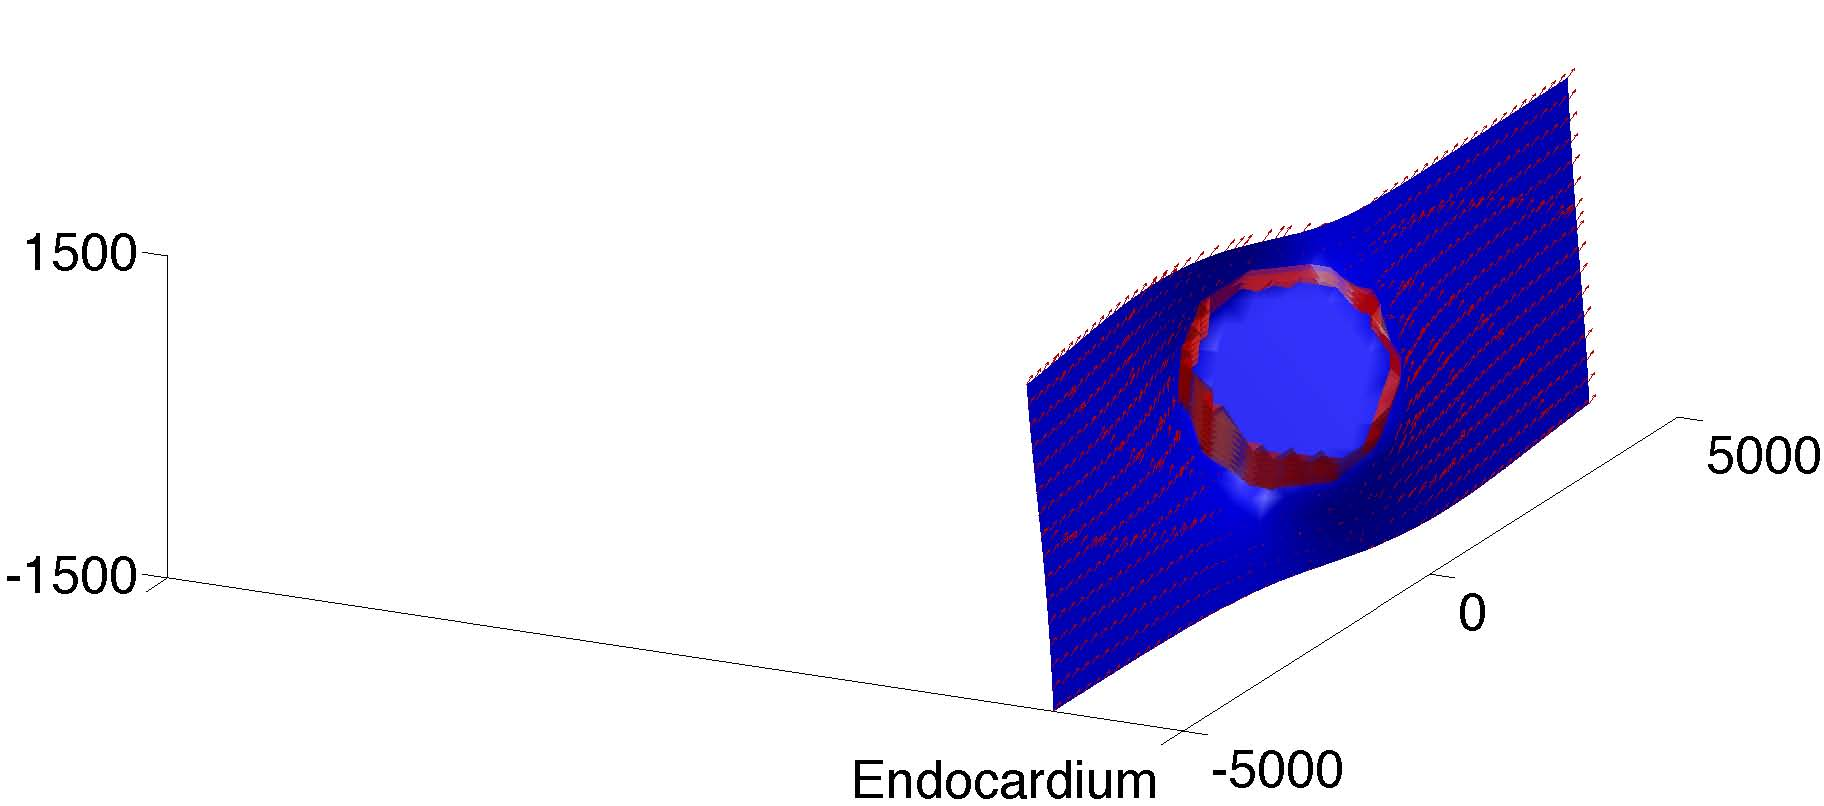
\includegraphics[width=1\textwidth]{Ch4/Figs/fibres_vessel2}} 
      \subfigure[][]{\label{fig:oblique_vessel3}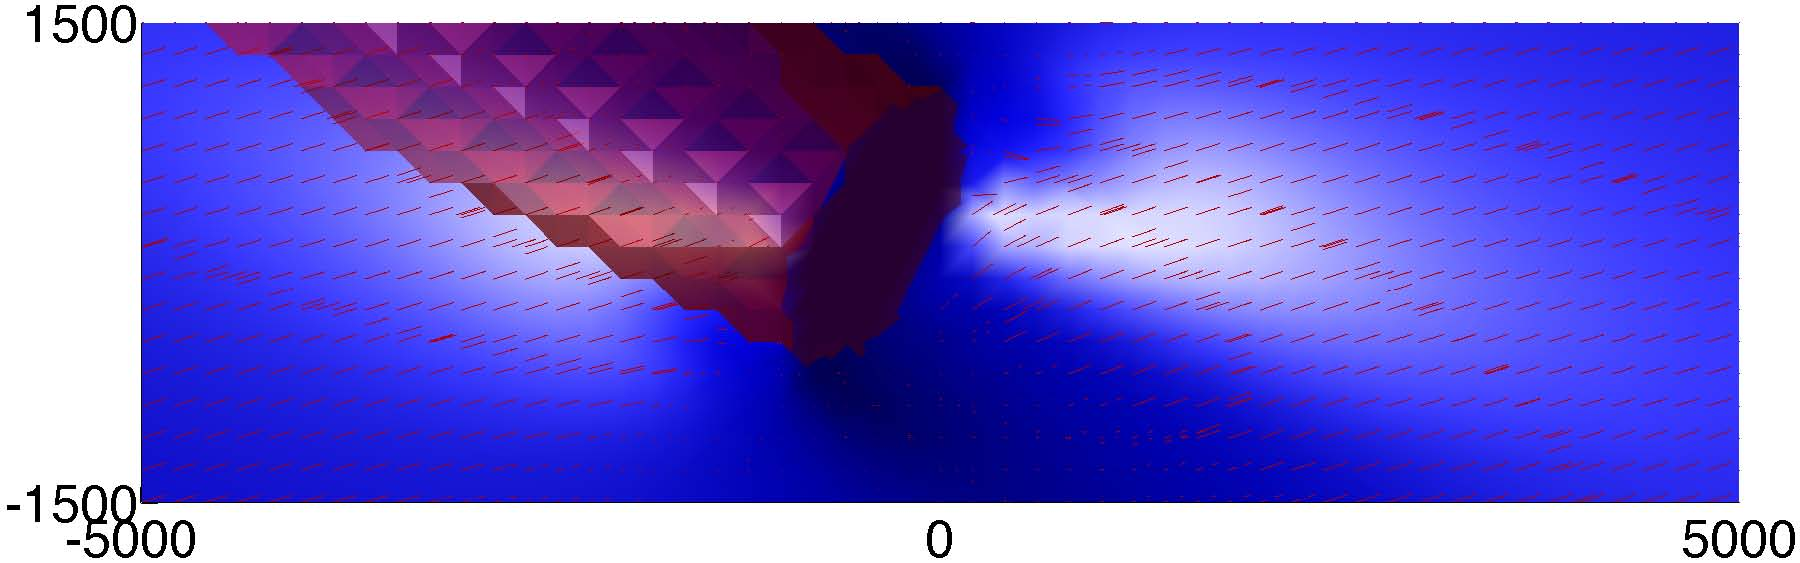
\includegraphics[width=1\textwidth]{Ch4/Figs/fibres_vessel3}}
      \caption{Three views of a vessel of radius 1mm, intersecting a myocardial lamina obliquely. Note the defomration of the sheet to accommodate the vessel, whilst minimising the area of the hole in its surface to $\pi r^2$ and the hole edge length to $2\pi r$. The fibre directions at various grid points on the lamina are also rendered, and can be seen more clearly in Figure~\ref{fig:oblique_no_vessel}.}
      \label{fig:oblique_vessel}
    \end{figure}

    \begin{figure}[htbp]
      \centering
      \vspace{-2.5em}
      \subfigure[][]{\label{fig:oblique_no_vessel1}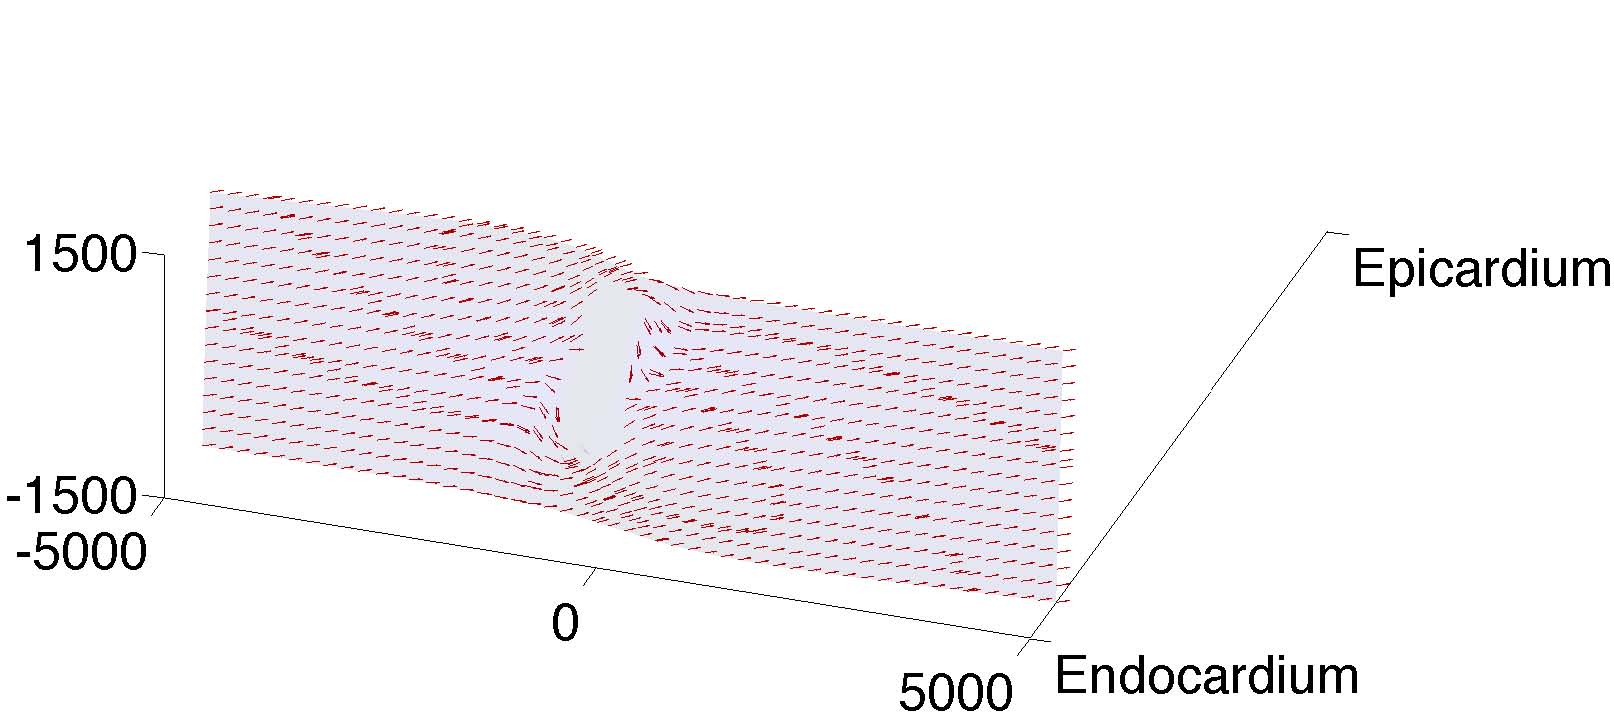
\includegraphics[width=1\textwidth]{Ch4/Figs/fibres_no_vessel1}}
      \subfigure[][]{\label{fig:oblique_no_vessel2}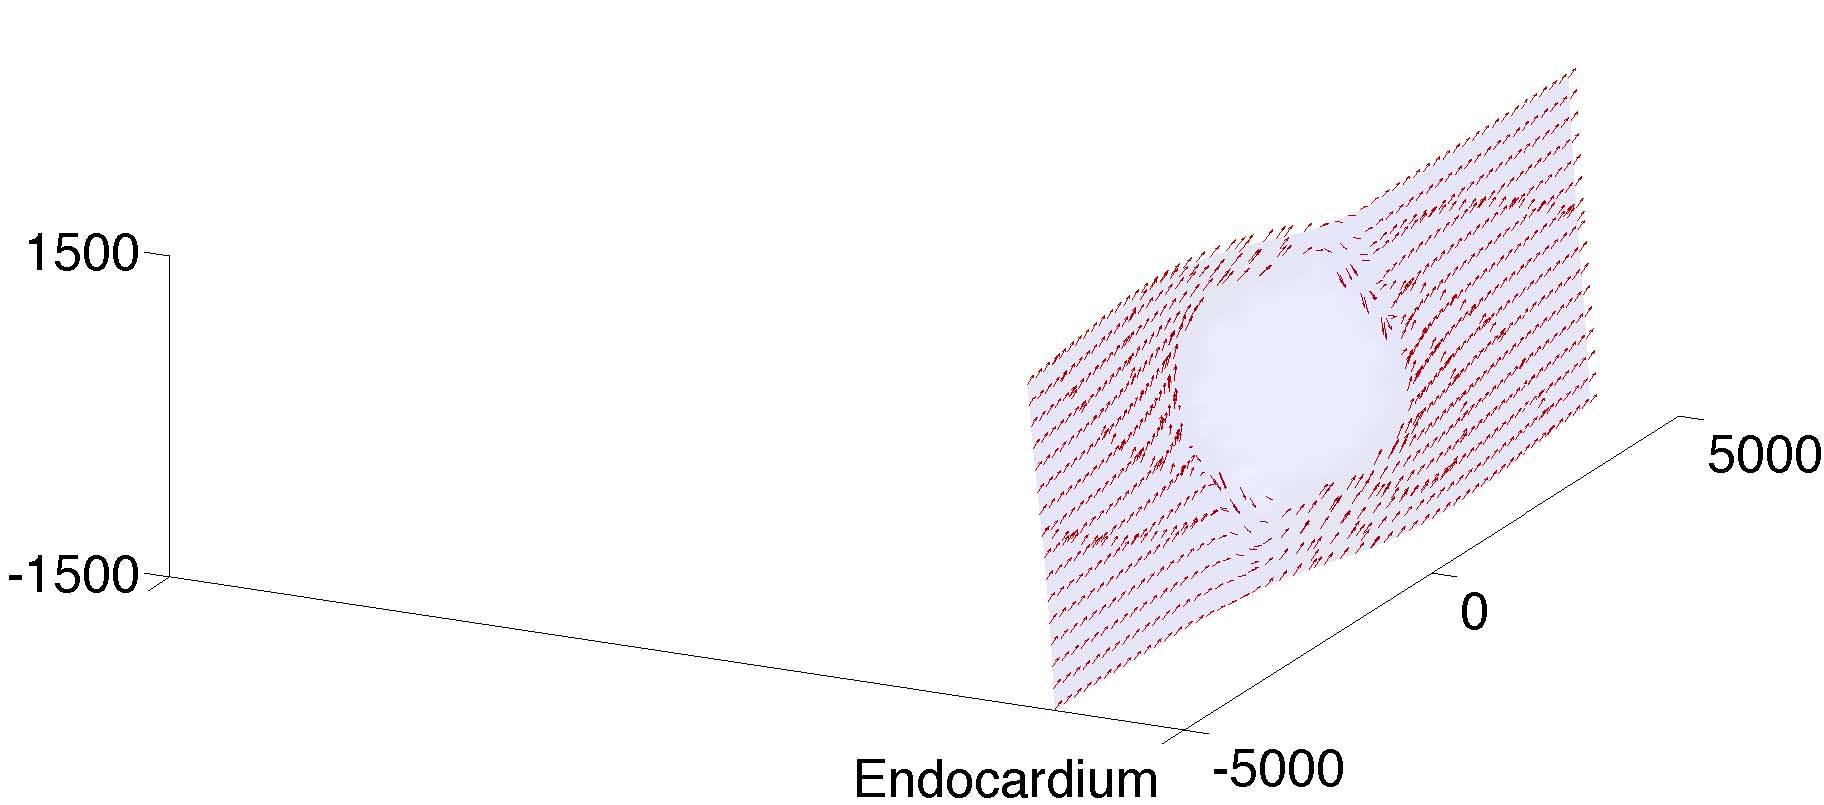
\includegraphics[width=1\textwidth]{Ch4/Figs/fibres_no_vessel2}} 
      \subfigure[][]{\label{fig:oblique_no_vessel3}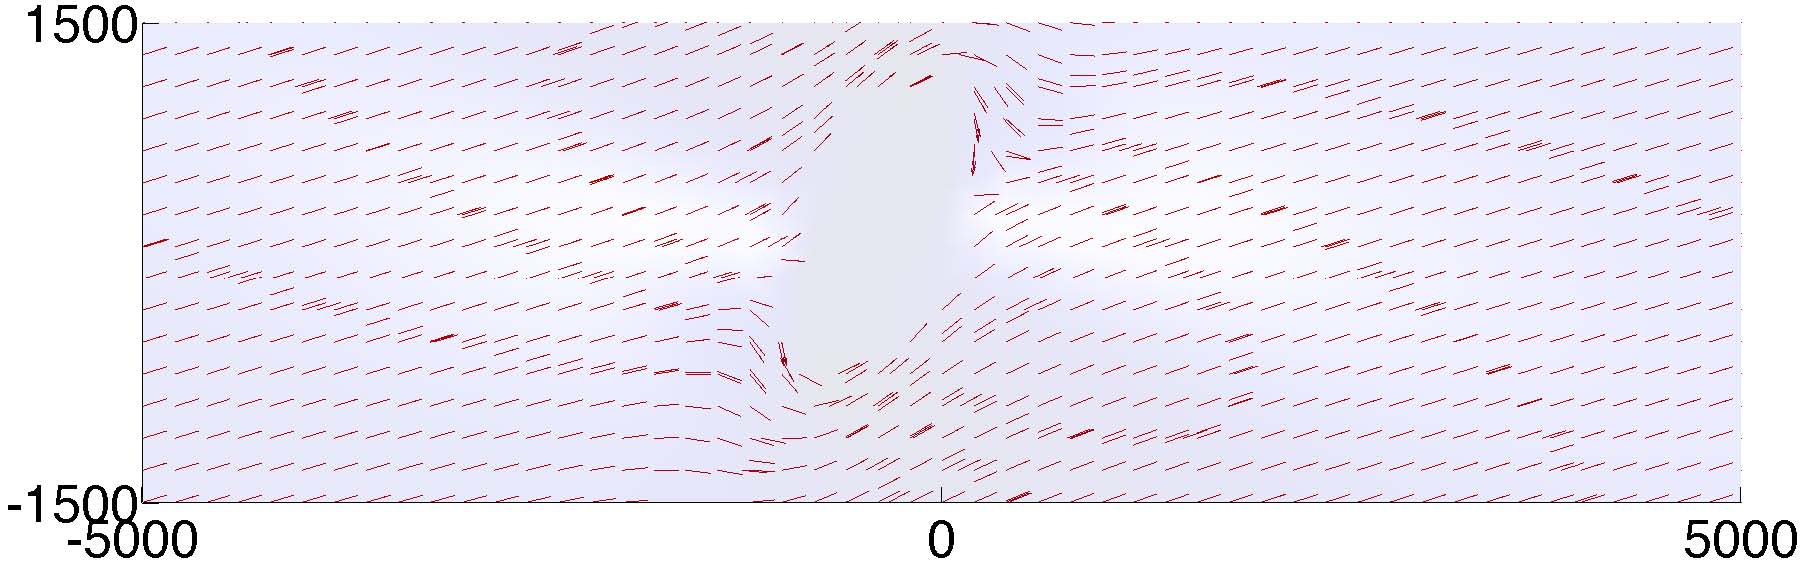
\includegraphics[width=1\textwidth]{Ch4/Figs/fibres_no_vessel3}}
      \caption{The same three views of the same vessel displayed in Figure~\ref{fig:oblique_vessel}, but with no vessel rendering and translucent lamina rendering, in order to display the fibre vectors clearly. From all angles, the fibres can be seen spreading around the vessel close to its boundary. A lamina close to the endocardium is visualised, and an overall $\alpha$ angle of $\sim20^\circ$ is observed away from the vessel.}
      \label{fig:oblique_no_vessel}
    \end{figure}
  
\subsection{Mesh Generation} % (fold)
\label{sec:mesh_generation}
  Binary voxel images of cuboid segments of tissue were generated in Matlab, with 0 representing the presence of tissue and 1 its absence. Initially, the open source program TetGen (tetgen.berlios.de) was used to process the array and generate tetrahedral meshes.
  
  The four points of a tetrahedron define a unique circumsphere. The ratio of the radius of this circumsphere to the shortest edge of the tetrahedron can be used as a quality constraint on the tetrahedra of any mesh. Even with maximum volume and radius-edge ratio constraints, the resulting TetGen (\url{tetgen.berlios.de}) meshes were irregularly arranged and shaped. An example of this irregular meshing can be seen in Figure~\ref{fig:tetgen}. It was decided instead to generate meshes with a piece of proprietary software called Tarantula (\url{www.meshing.at}). Figure~\ref{fig:tarantula} is in stark contrast to Figure~\ref{fig:tetgen}; the Tarantula mesh is nearly entirely regular, apart from a pattern of switching between the orientations of the tetrahedra that make up cubic mesh segments.
  
  \begin{figure}[htbp]
    \centering
    \subfigure[][A 10x10x3mm mesh generated from a 100$\mu$m resolution voxel image with {[0,0,1]} vessel direction and 1mm radius.]{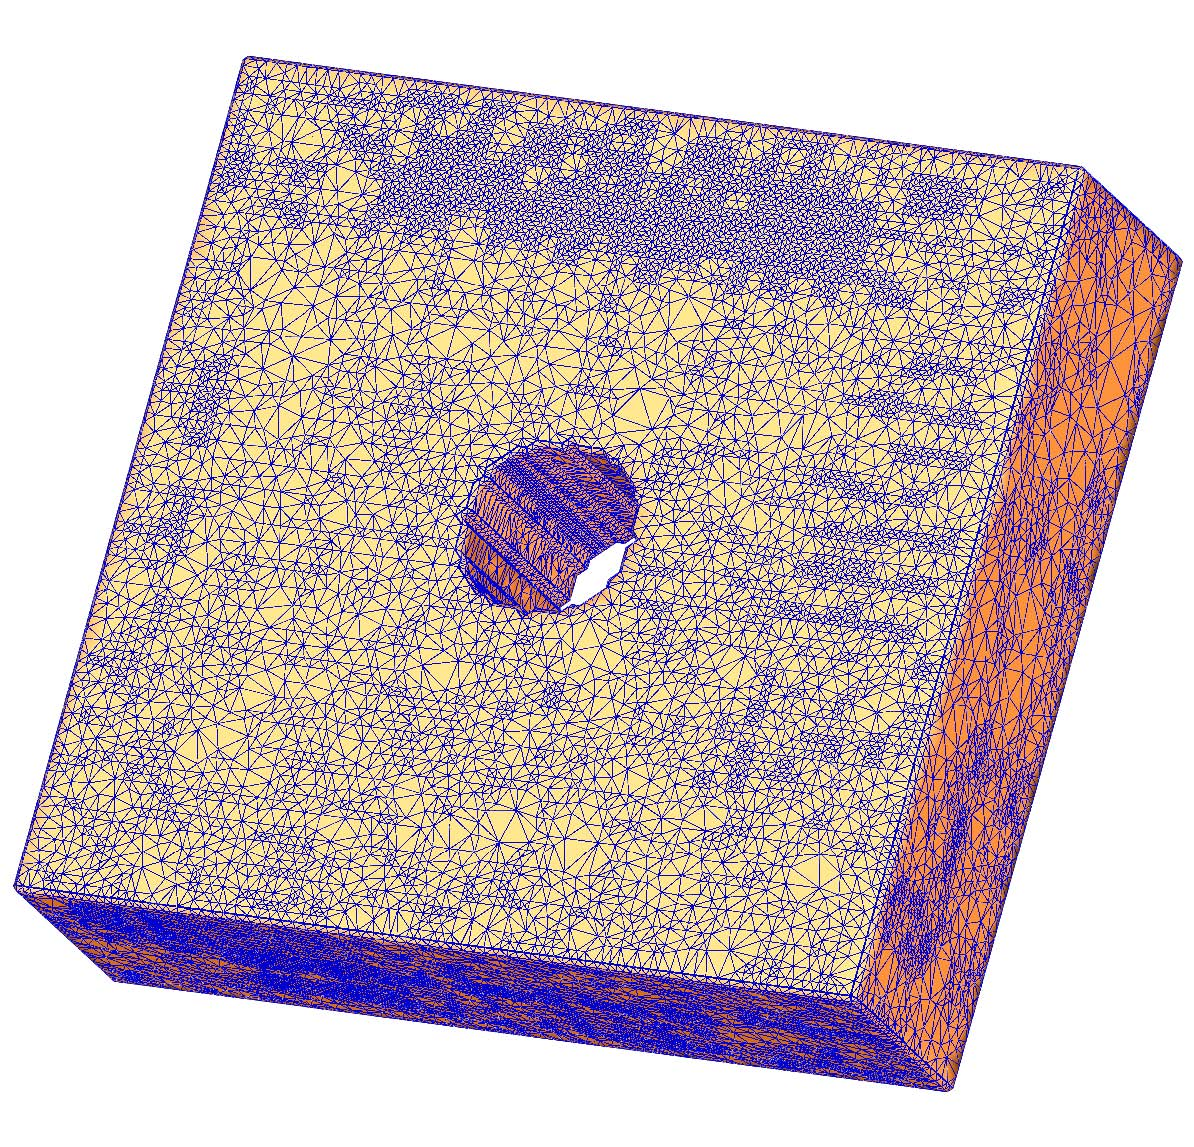
\includegraphics[width=0.6\textwidth]{Ch4/Figs/tetgen}}
    \subfigure[][An enlarged view of the same mesh.]{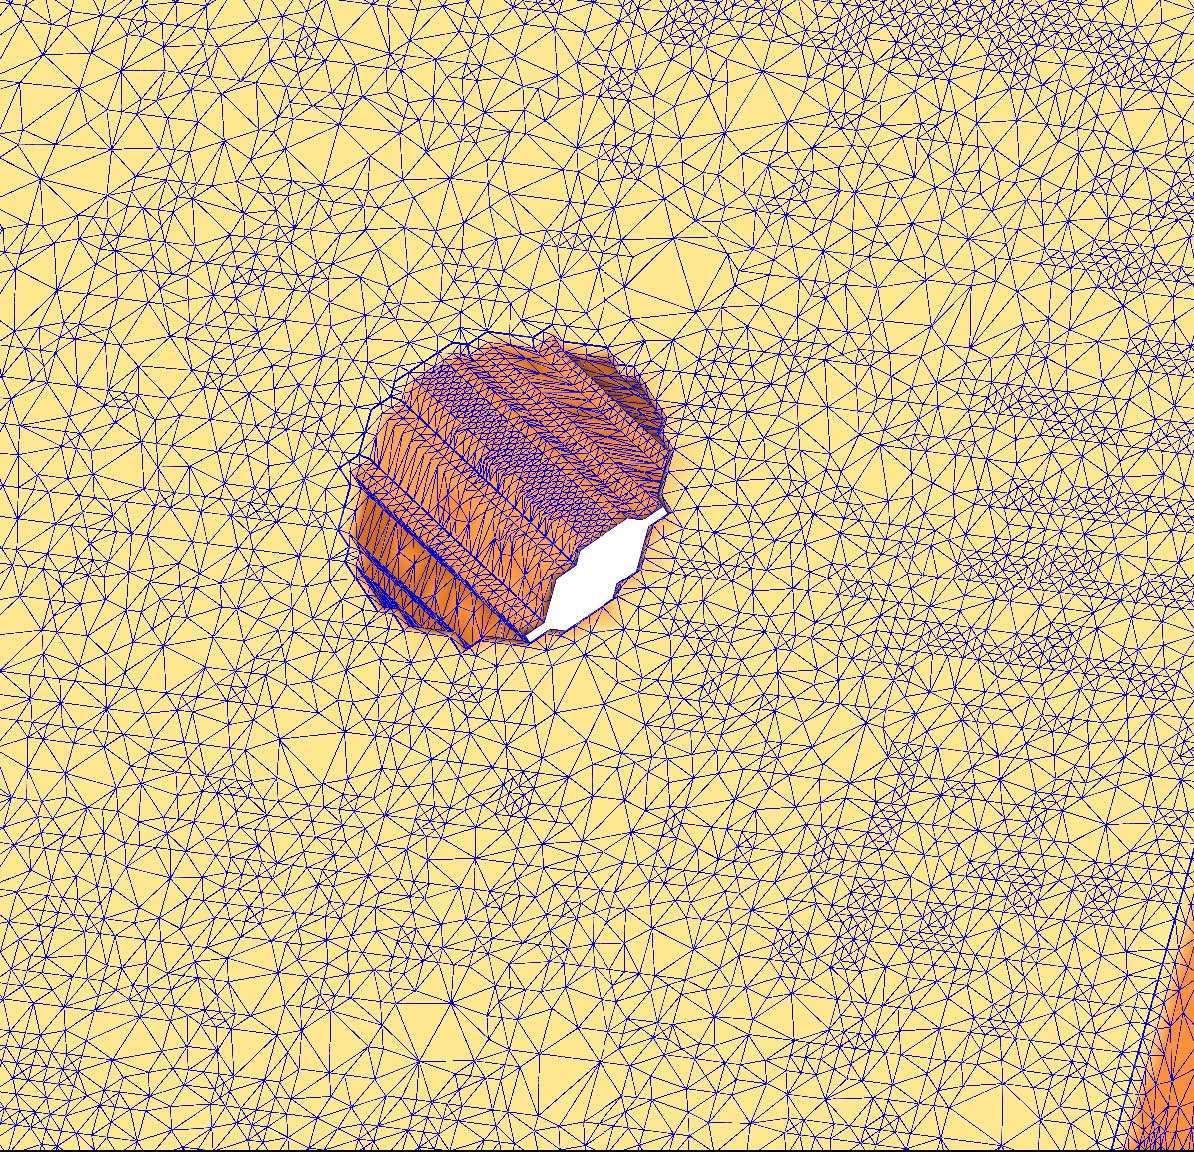
\includegraphics[width=0.6\textwidth]{Ch4/Figs/tetgen_zoom}} 
    \caption{An example of a mesh generated by TetGen and visualised in Meshalyzer (part of the CARP package). Despite a regular, symmetrical input node array, the mesh is very irregular, with seemingly inexplicable patches of dense tetrahedralisation. The long thin tetrahedra at the edges of the tissue associated with bad mesh quality have been replaced with several smaller ones, but the mesh is still far from ideal.}
    \label{fig:tetgen}
  \end{figure}
  
  \begin{figure}[htbp]
    \centering
    \subfigure[][]{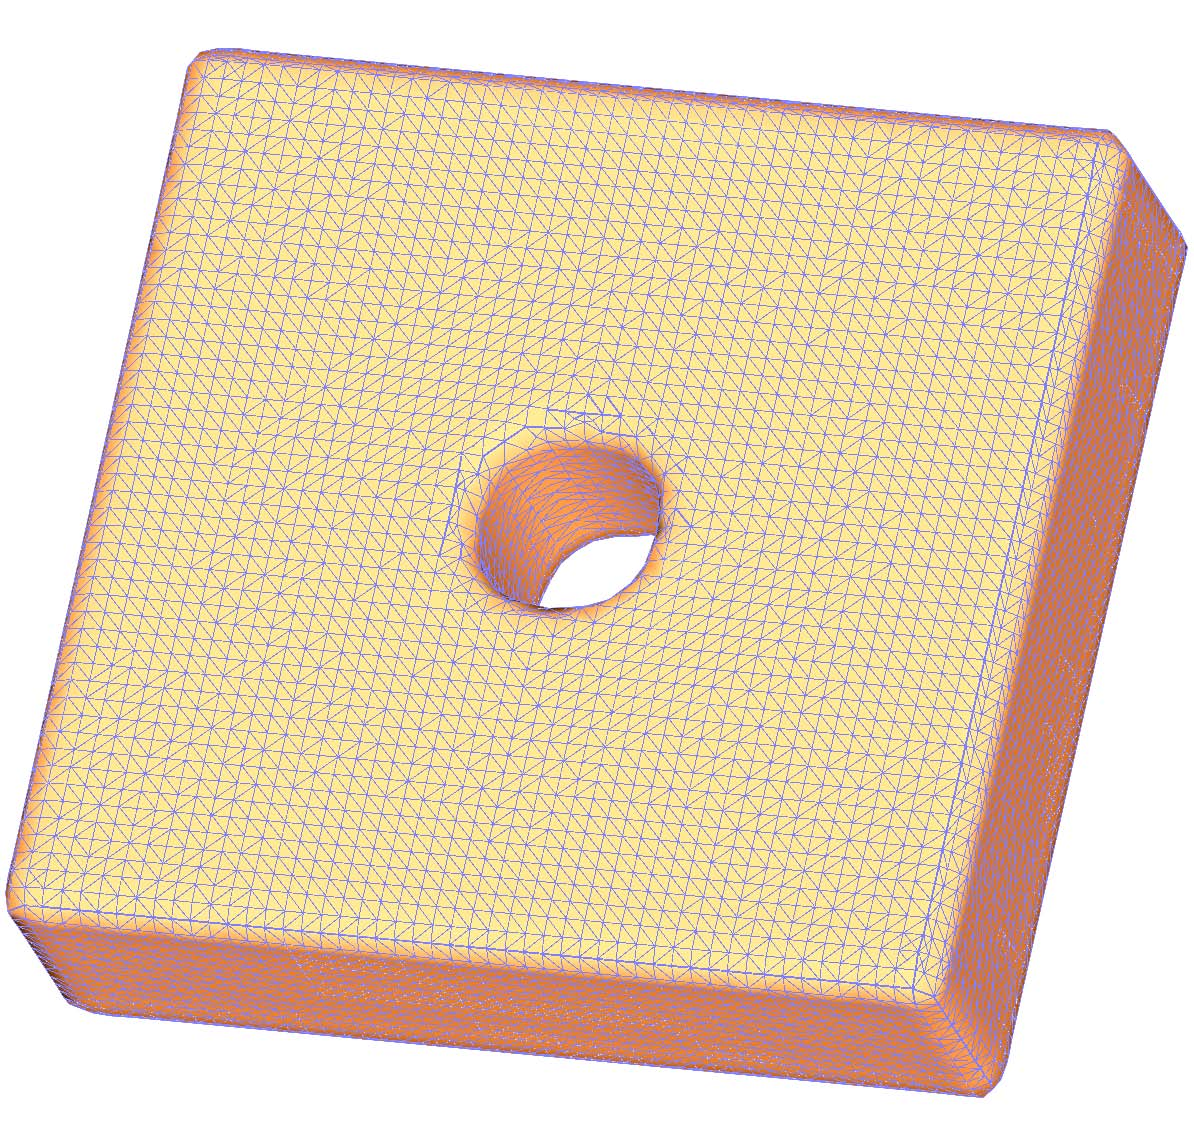
\includegraphics[width=0.6\textwidth]{Ch4/Figs/tarantula}}
    \subfigure[][]{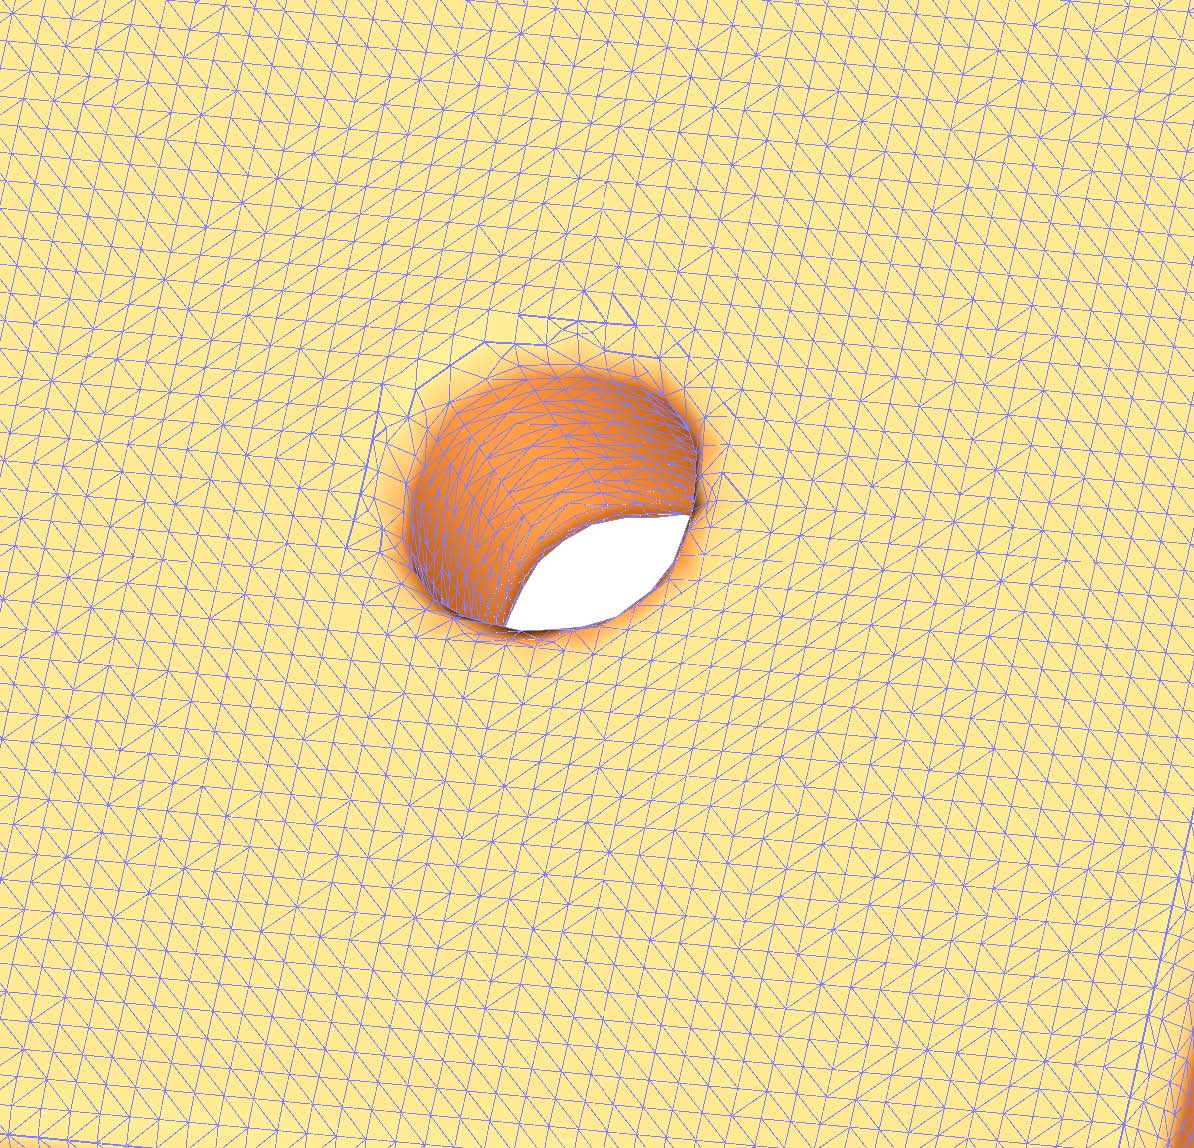
\includegraphics[width=0.6\textwidth]{Ch4/Figs/tarantula_zoom}} 
    \caption{An example of a mesh generated by Tarantula. This mesh is clearly much more regular than that of Figure~\ref{fig:tetgen} and was used in simulation. The mesh constitutes 50,000 nodes and approximately 270,000 tetrahedral elements.}
    \label{fig:tarantula}
  \end{figure}
  
  There were several formatting issues associated with the final workflow. Once Tarantula had generated a tetrahedral mesh from the voxel image file built in Matlab, a C++ script written by Anton Prassl was used to convert the various Tarantula file formats so that they could be interpreted by the electrophysiological simulation package CARP (Cardiac Arrhythmias Research Package) \cite{Vigmond2003}. Tarantula generates both an intracellular (tissue) mesh and a surrounding extracellular box, so CARP was then used to extract just the intracellular space from the total mesh, for the purposes of monodomain simulations.
  
\subsection{Evaluating the Fibre Direction at the Element Centroids} % (fold)
\label{sec:evaluating_the_fibre_direction_at_the_element_centroids}
  The final step before running simulations was to use the model from sections~\ref{sec:defining_the_laminae_of_equal_helical_angle} and \ref{sec:defining_the_fibre_direction_within_the_laminae} to calculate the fibre directions at the centre of each tetrahedron. Given the coordinates of each of the four vertices of a tetrahedron $\mathbf{p}_i$, the formula for the centroid is
  
  \begin{equation}
    \mathbf{p}_{\text{centroid}} = \frac{\mathbf{p}_1+\mathbf{p}_2+\mathbf{p}_3+\mathbf{p}_4}{4} .
  \end{equation}
  
\subsection{Mesh Dimensions} % (fold)
\label{sub:mesh_dimensions}
  It is observed from the extracted vasculature in Figure~\ref{fig:vessels} that the major myocardial vessels are sub-epicardially or transmurally oriented: they lay either along the outer surface of the heart, or sink directly through the heart wall. The largest of the vessels, for example the coronary artery, are approximately 2mm in diameter.
  
  \begin{figure}[htbp]
		\centering
		\subfigure[][Vertical MRI slice.]{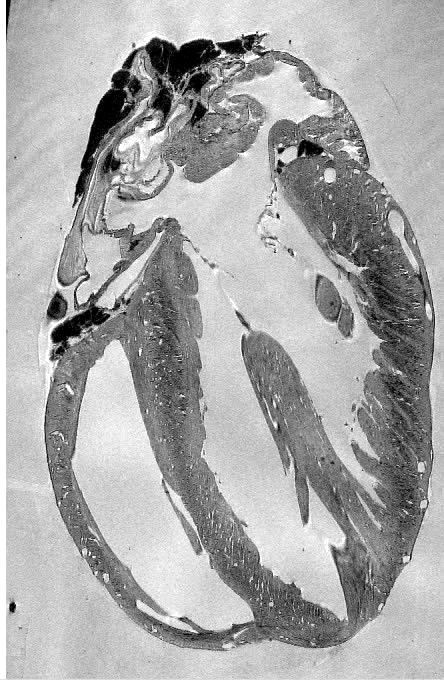
\includegraphics[height=51ex]{Ch4/Figs/vertical_mri}}
		\qquad
    \subfigure[][Extracted vascular tree.]{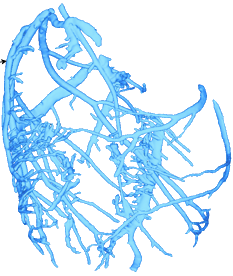
\includegraphics[height=51ex]{Ch4/Figs/extracted_vessels}}
    \caption{\textbf{(a)} A 2D image in the coronal plane from a 3D Rabbit MRI dataset at resolution $26.4\times26.4\times24.4\mu$m from \cite{Burton2006}. Circular and elliptical cavities distributed within the myocardium can be observed.  These are the major vessels supplying the heart. \textbf{(b)} The vascular tree was extracted from the MRI dataset by Bishop et al \cite{Bishop2009}. The main vessels are positioned either sub-epicardially or transmurally.}
	  \label{fig:vessels}
	\end{figure}
  
  With these findings in mind, meshes were generated that contained a 2mm vessel, either spanning from endocardium to epicardium, or situated parallel to the epicardium, 0.5mm from the surface. In the following sections we consider two sets of experimental protocol: first, a pair of square 10 x 10 x 3mm meshes to which a single stimulus was applied, inducing a planar wave that progresses once across the domain; and second a wider, 35 x 10 x 3mm mesh, where a first stimulus induces a planar wave and precedes a second stimulus triggers an artificial arrhythmic episode in the wake of the wave. It is noted that all meshes measure 10mm in the $y$-direction, in accordance with the approximate width of left-ventricular rabbit heart wall.
% subsection mesh_dimensions (end)

\subsection{Electrophysiological Simulation} % (fold)
\label{sec:electrophysiological_simulation}  
  Once each tetrahedron has been assigned a conductivity tensor, based on the modelled fibre direction at its centroid, simulations were run in CARP, using the UCLA rabbit ventricular action potential model \cite{Mahajan2008}. CARP was chosen because at the time, it was the only cardiac simulation package that fully supported bidomain simulations. Simulations were run in parallel on the Oxford OeRC cluster and took approximately a few hundred seconds to compute 300ms of activation on 32 cores.
  
% section methods (end)

\section{Results} % (fold)
\label{sec:results}
  \subsection{Planar Propagation} % (fold)
  \label{sub:planar_propagation}
    The first set of simulations aimed to clarify the differences in propagation dependent on four sets of binary criteria: transmural or sub-epicardial vessel orientation; a transmural or circumferential wave propagation direction; the usage of a bidomain or monodomain model; and the implementation of a simple or an accurate fibre model. Simulations based on each of the 16 points in this discrete space are arranged in a table in Figures~\ref{fig:planar_propagation_1} and \ref{fig:planar_propagation_2}. Perhaps the most striking difference in the figures is the speed of propagation between the transmural and circumferential protocols. The wave is comparatively retarded in the top half of the tables, as it travels from the endocardium at the bottom edge of the cuboid, to the epicardium at the top edge. Regardless of transmural variation in fibre direction, this vertical direction is always perpendicular to the fibres, resulting in minimum conduction speed. Contrastingly, the transmural variation is evident in the bottom half. As the wave travels fastest through the central horizontal band of the mid-myocardium, where the fibres point from left to right, conduction is slower near the muscle walls, where the fibres are more transverse to the propagation direction.
    
    The two criteria of vessel orientation and stimulation protocol separate the tables into 4 sub-squares. It is only meaningful to compare activation times of a particular tetrahedron, a particular point in the tissue, in two simulations from the same sub-square, where both the mesh and the stimulation protocol are the same. Each subsquare is divided again by domain and fibre models. It is just visible from the two figures that monodomain waves propagate slightly faster than their bidomain partners, yet no discernable qualitative difference was found between the two regimes, and so since monodomain computation was faster by an order of magnitude or more, it was decided to use monodomain from here onwards. Differences were observed, however, between the accurate and simple fibre orientation models in all cases, the significance of which depended upon both the orientation of the vessel and the direction of propagation of the wavefront. Figure~\ref{fig:difference_maps} arranges the four monodomain time difference maps between the simple and accurate fibre models. Activation times differed only slightly during transmural stimulation around a transmural vessel (top left of Figure~\ref{fig:difference_maps}), in the only scenario where propagation direction was parallel to vessel orientation. Larger timing differences can be seen in the region surrounding the vessels in the other three maps. We see slower reds before the wave hits the vessel, but faster blues and even blacks in the vessel wake, indicating that the negotiationg fibres have guided the wavefront around the vessel faster than in the simple model. Indeed, during cirumferential stimulation across an epicardial vessel (bottom right of Figure~\ref{fig:difference_maps}) a maximum difference in activation time of -4ms was observed just behind the vessel in blue, and an elongated blue wake extends from the vessel to the right. This demonstrates that wavefront curvature induced by the presence of the vessel was sustainedly more severe in the accurate model than in the simple.
    
    \begin{figure}[htbp]
  		\centering
  	    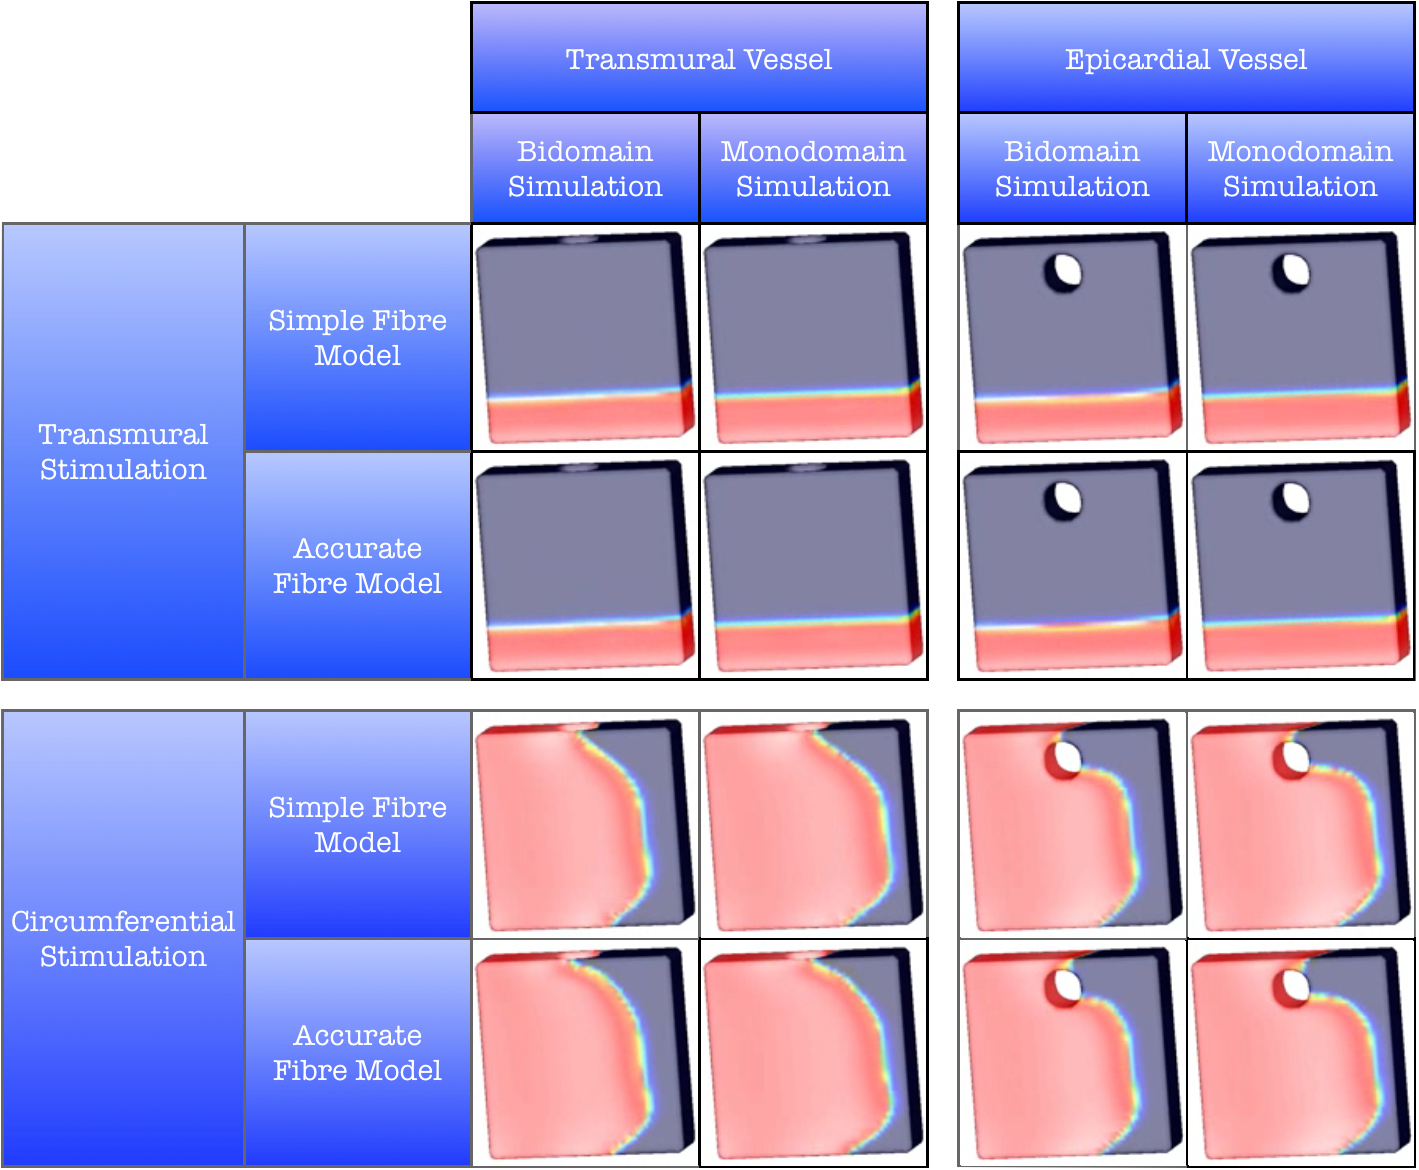
\includegraphics[width=1\textwidth]{Ch4/Figs/planar_propagation_1}
              \caption{An array of 16 simulated electric waves on 10 x 10 x 3mm cuboid meshes. Each simulation is initialised with 5ms of externally applied shock, along either the bottom or left edge of the domain. The resulting waves are displayed at 160ms. Black areas represent fully polarised tissue which has yet to be stimulated, red and white areas represent fully depolarised tissue, and just visible at the wavefronts are the blue, green and yellow spectra in between, representing tissue in the upstroke phase. It is clear that the left-hand two columns are simulations of a transmural vessel, and the right hand columns of an epicardial vessel. In the top two rows, a wave has been stimulated from the bottom of the diagrams, the endocardium, to the top, at the epicardium, but in the bottom two rows a wavefront is stimulated that propagates from the left of the diagrams over to the right. The snapshots are further divided into monodomain and bidomain simulations, and into simple and accurate fibre modelling.}
  	  \label{fig:planar_propagation_1}
  	\end{figure}
    
    \begin{figure}[htbp]
  		\centering
  	    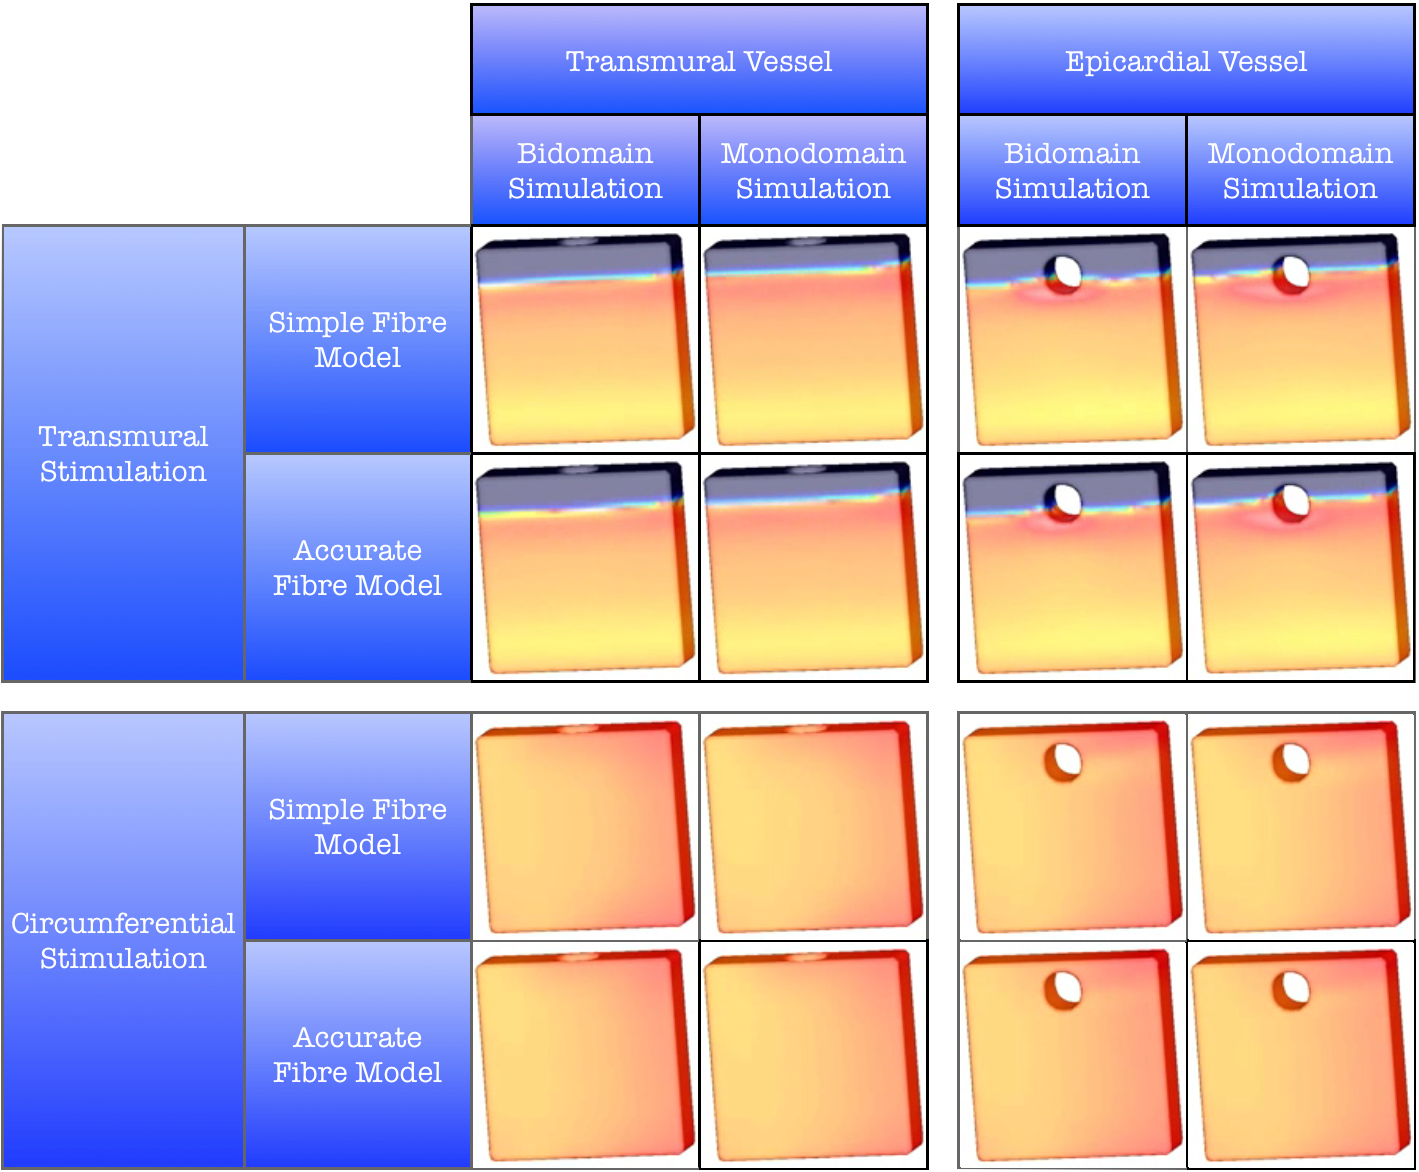
\includegraphics[width=1\textwidth]{Ch4/Figs/planar_propagation_2}
              \caption{The same array of simulations as displayed in Figure~\ref{fig:planar_propagation_1}, the waves being displayed at the later time of 270ms, in order to show the interaction of the epicardial vessel with the wavefront.}
  	  \label{fig:planar_propagation_2}
  	\end{figure}

    \begin{figure}[htbp]
  		\centering
  	    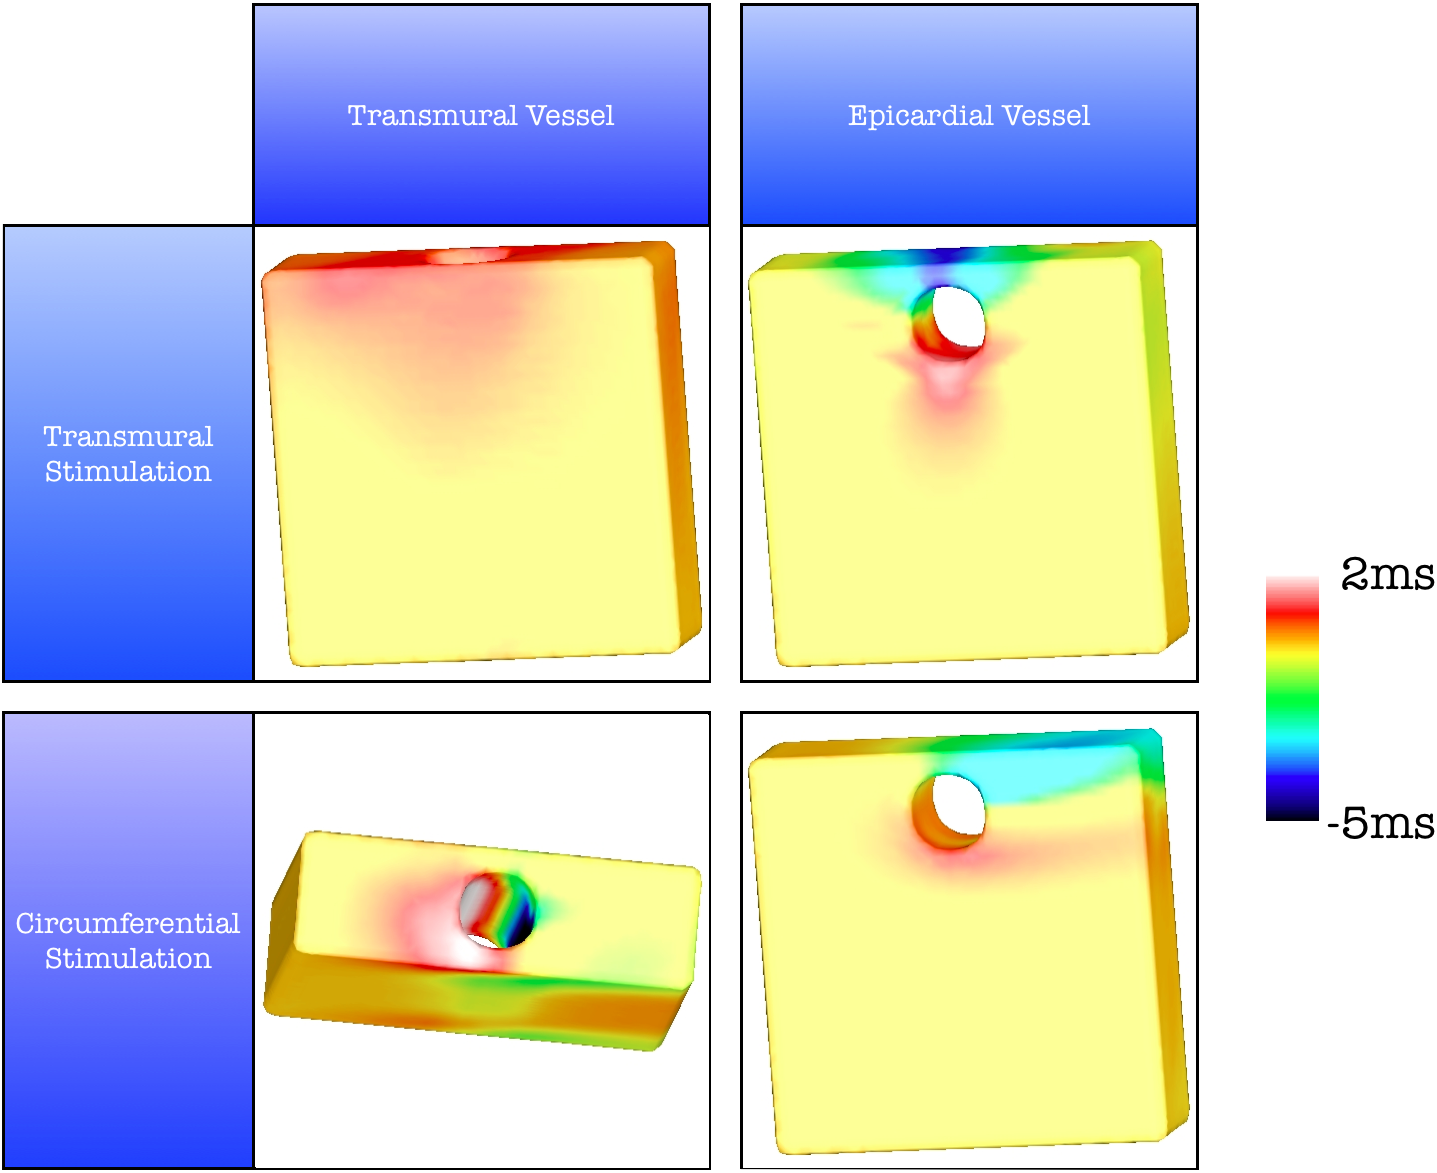
\includegraphics[width=0.95\textwidth]{Ch4/Figs/difference_maps}
              \caption{Four difference maps comparing the time of first stimulation in the simple and accurate fibre models, for both propagation directions and both vessel orientations. The monodomain models were used in all cases. Times from the simple fibre model are subtracted from those of the accurate model, so that positive values represent a longer time until first stimulation in the accurate model, and negative values signify a faster stimulation. The scale is shown on the right: yellow means no time difference, reds and whites mean a delay in the accurate model compared to the simple model, and the greens and blues in the top right mean quicker activation times in the accurate model. A view of the epicardial edge is presented in the bottom left map, in order to show strong deviations on the inner vessel wall.}
  	  \label{fig:difference_maps}
  	\end{figure}
  	
  
  \subsection{Induced Arrhythmia} % (fold)
  \label{sub:induced_arrhythmia}
    Where the first stage of experiment aimed to demonstrate possible arrhythmogenic mechanisms, acting through the increase in wave curvature due to vessels, this next stage examined the role of vessels and fibres once an arrhythmia was in progress. Since mapping studies \cite{Valderrabano2003,Cysyk2008,Qin2005} attributed phase singularity anchoring to epicardial vessels, we initiated singularities around an epicardial vessel, on a domain large enough to contain an arrhythmia meandering in the vicinity of the vessel. The extended 35 x 10 x 3mm mesh was subject to a double stimulation protocol: for the first 5ms, the bottom edge was shocked to initiate a transmural wave, much in the manner adopted in section~\ref{sub:planar_propagation}; then after 600ms, one half of the tissue between the vessel and the endocardium is shocked, triggering a reentrant spiral wave. Figures~\ref{fig:shock_induced_54ms}--\ref{fig:shock_induced_2160ms} chronicle the double stimulation and subsequent arrhythmic episode for both fibre models. Both vessels reveal some anchoring effect, but it is stronger and perpetuated for longer in the simple model, where vertical propagation at the vessel boundary is more strongly retarded. Wave breakup is also more pronounced, with more angular, fibrillatory waveforms visible.
  	
    \begin{figure}[htbp]
  		\centering
  	    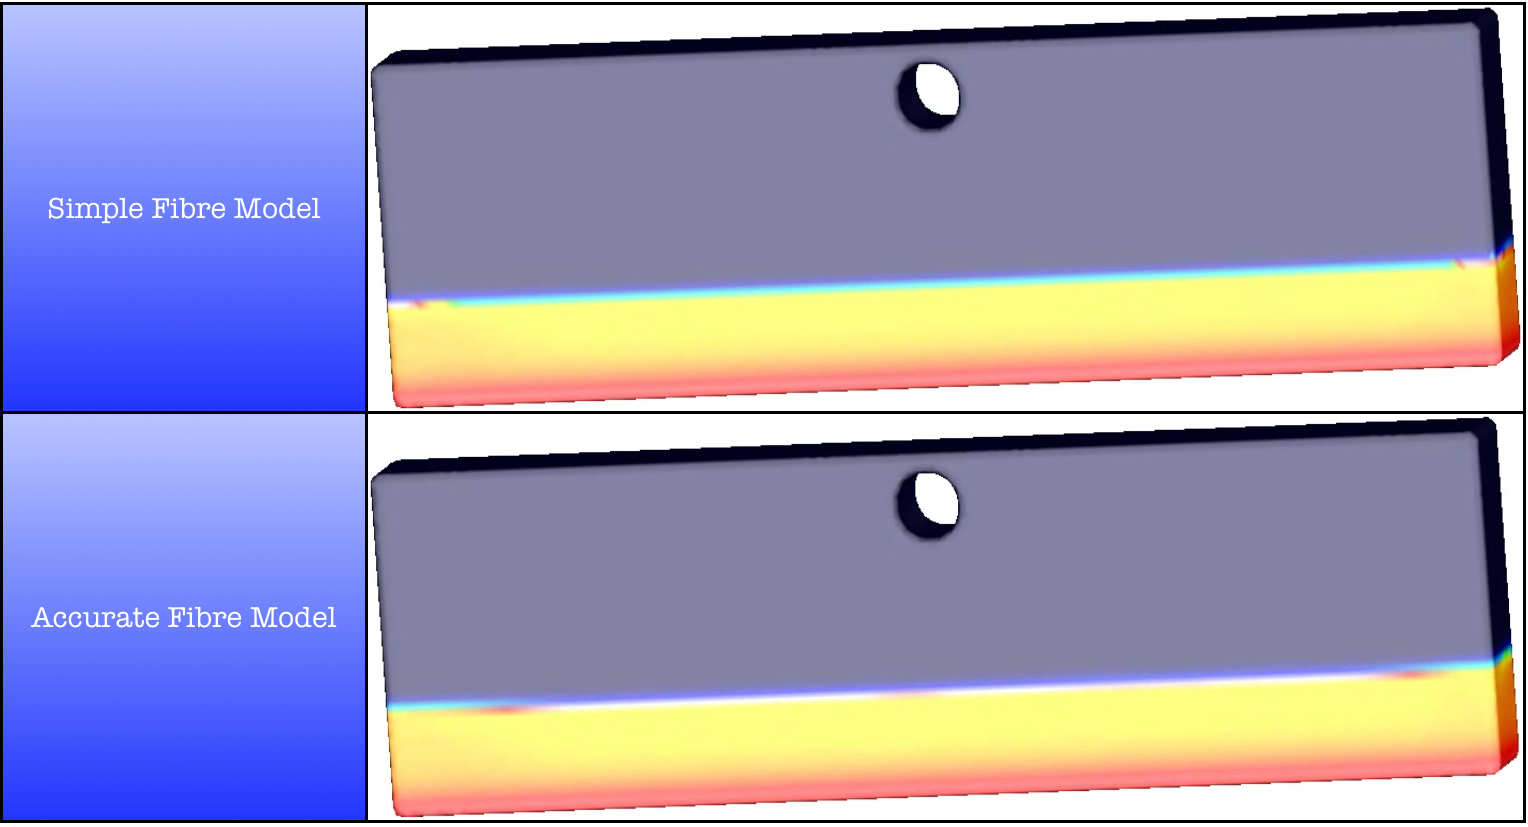
\includegraphics[width=0.95\textwidth]{Ch4/Figs/shock_induced_54ms}
              \caption{Monodomain simulations on a 35 x 10 x 3mm mesh representing a transmural section of rabbit left-ventricular heart wall around a 2mm sub-epicardial vessel. The two snapshots are taken 54ms after an endocardial stimulus. The simple fibre model is employed in the top snapshot, and the accurate in the bottom.}
  	  \label{fig:shock_induced_54ms}
  	\end{figure}
  	
    \begin{figure}[htbp]
  		\centering
  	    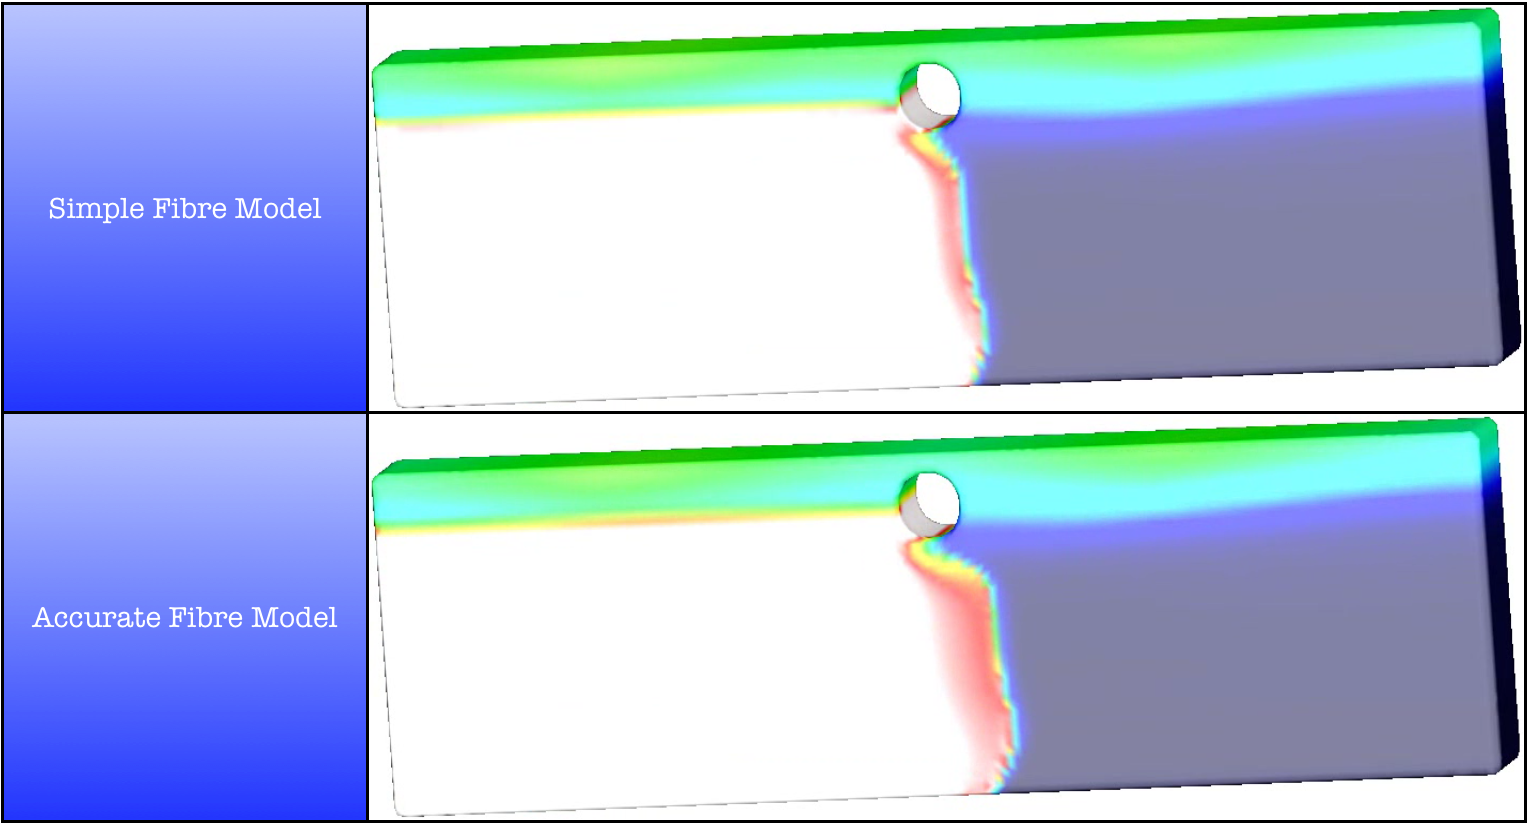
\includegraphics[width=0.95\textwidth]{Ch4/Figs/shock_induced_558ms}
              \caption{A second shock is applied at 558ms in order to induce arrhythmia. Green tissue above the shock zone has not recovered from the previous stimulation, and so conduction upwards is blocked. The wave will move laterally for a short time until the green band recovers and an anticlockwise spiral wave ensues.}
  	  \label{fig:shock_induced_558ms}
  	\end{figure}
  	
    \begin{figure}[htbp]
  		\centering
  	    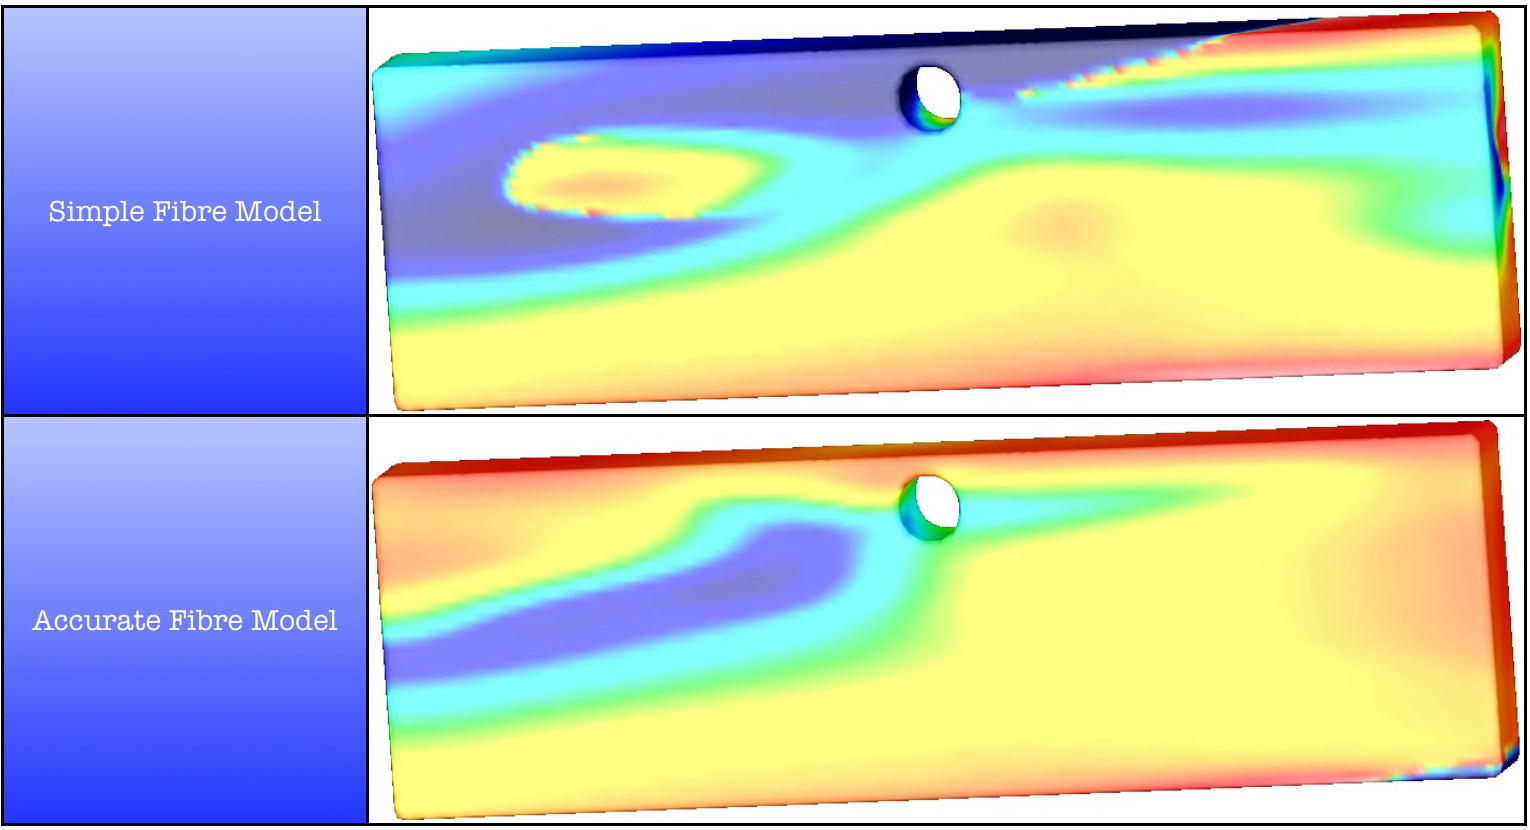
\includegraphics[width=0.95\textwidth]{Ch4/Figs/shock_induced_1530ms}
            \caption{At 1530ms, the accurate arrythmia (bottom) has dissipated and tissue will restore to a polarised state, whereas the simple arrhythmia has fractionated into several wavefronts, showing complex 3D dynamics.}
  	  \label{fig:shock_induced_1530ms}
  	\end{figure}
  	
    \begin{figure}[htbp]
  		\centering
  	    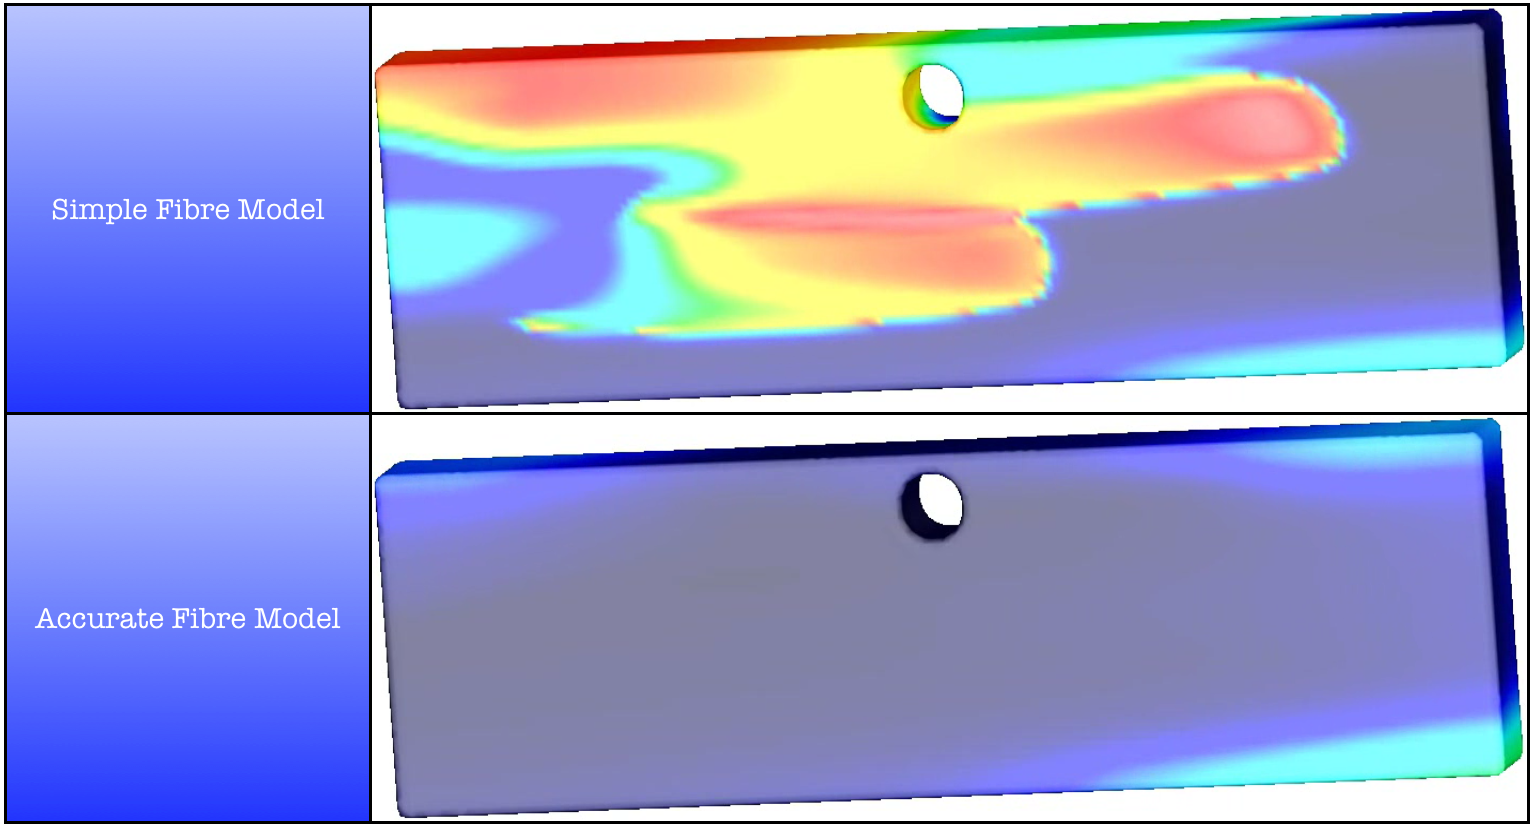
\includegraphics[width=0.95\textwidth]{Ch4/Figs/shock_induced_1710ms}
              \caption{At 1710ms, the simple arrhythmia exhibits several phase singularities, with one staying local to the vessel.}
  	  \label{fig:shock_induced_1710ms}
  	\end{figure}
  	
    \begin{figure}[htbp]
  		\centering
  	    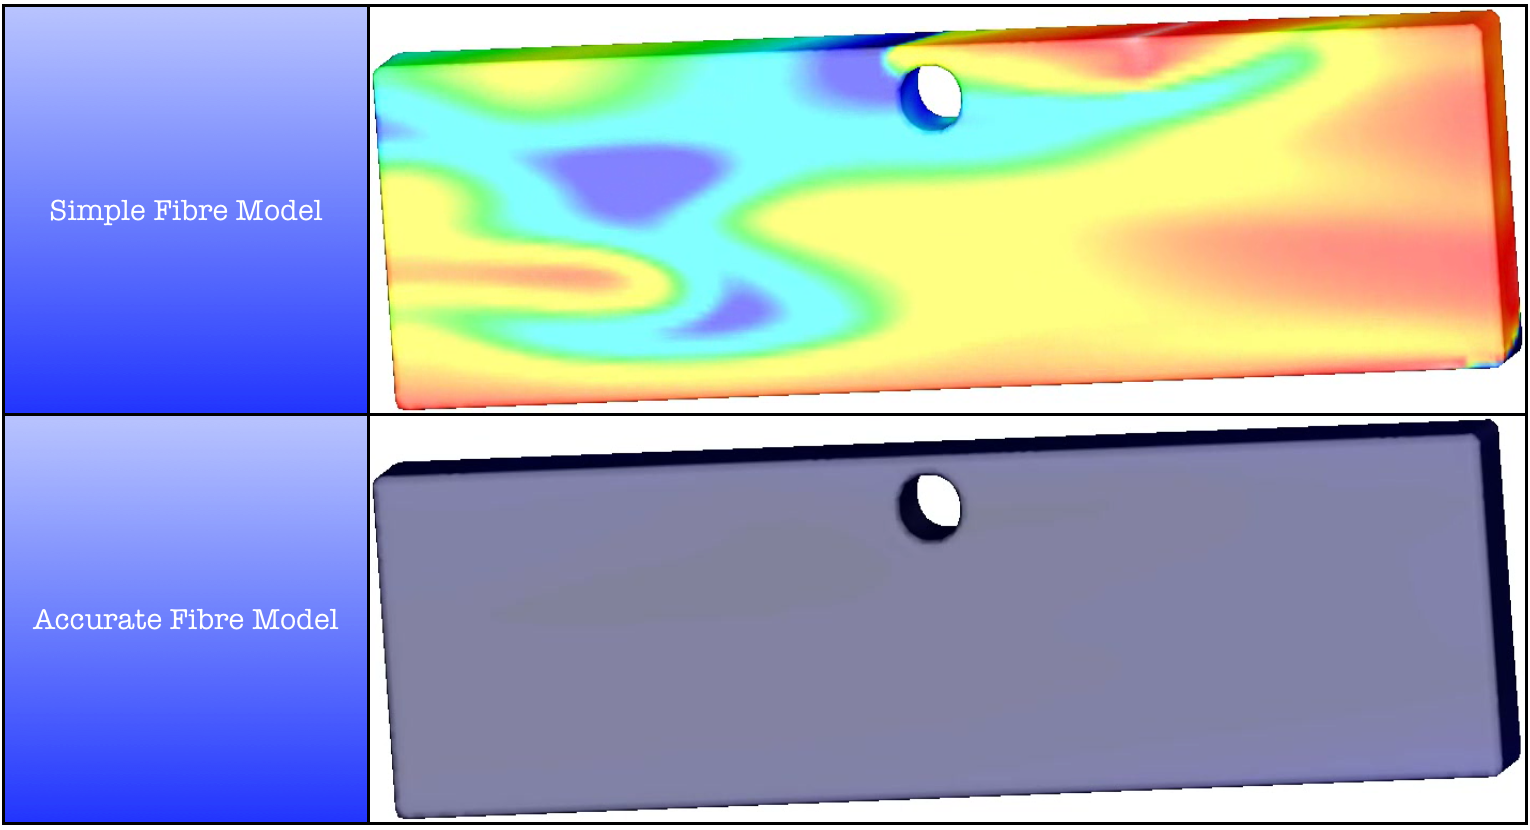
\includegraphics[width=0.95\textwidth]{Ch4/Figs/shock_induced_1890ms}
              \caption{At 1890ms, all but the anchored singularity are on the verge of extinction. The vessel extends the circuit length of the reentrant wave, allowing tissue to recover and reactivate when the wavefront returns. In the simple fibre model, the fibre direction remains horizontal at the vessel boundary, rather than tangent to the boundary. Propagation is thus significantly retarded in the vertical direction to the left and right of the vessel. This effect further extends the effective circuit length.}
  	  \label{fig:shock_induced_1890ms}
  	\end{figure}
  	
    \begin{figure}[htbp]
  		\centering
  	    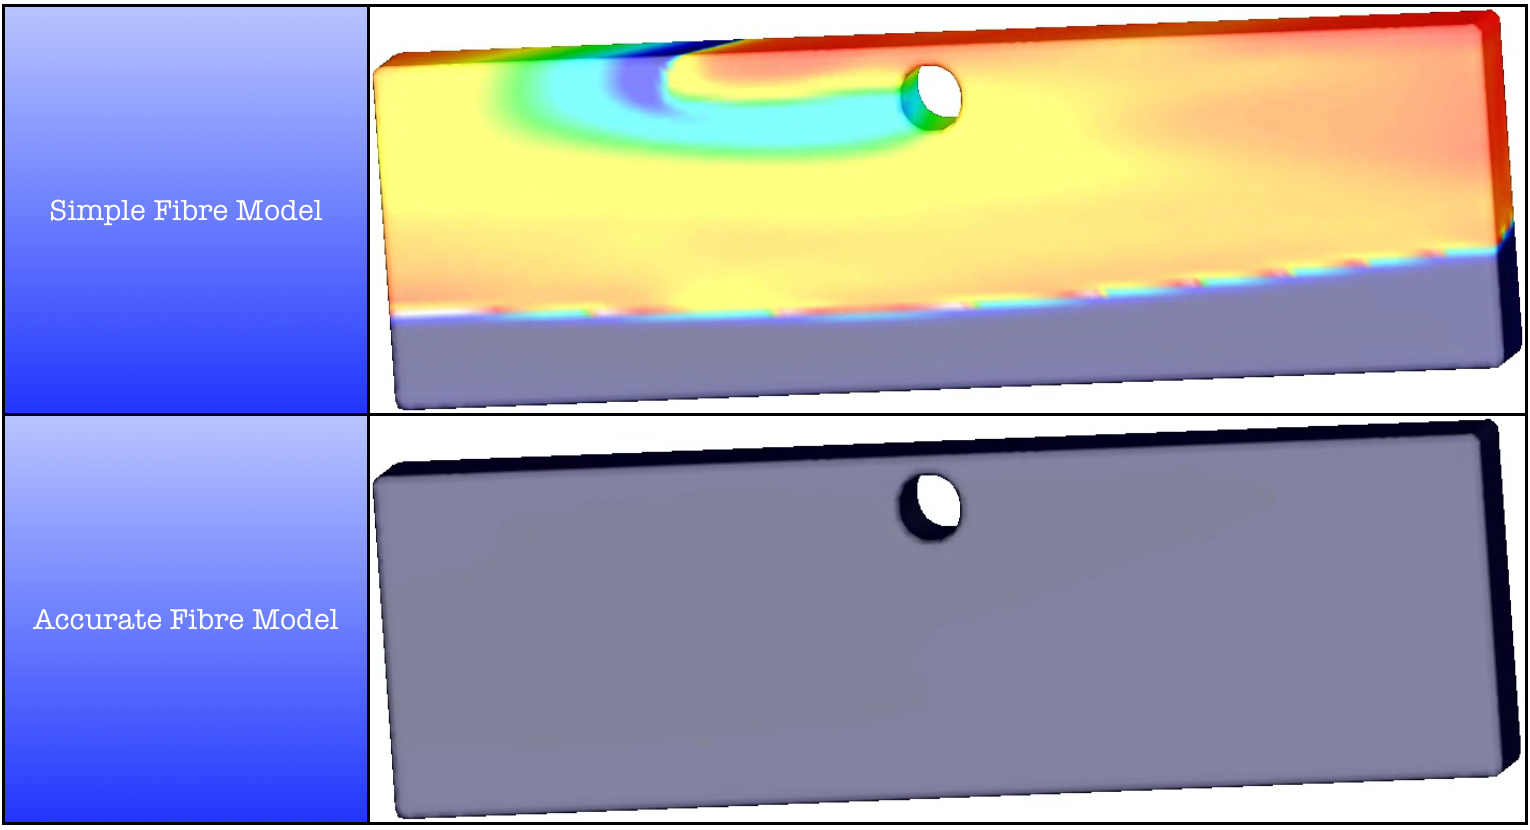
\includegraphics[width=0.95\textwidth]{Ch4/Figs/shock_induced_2160ms}
              \caption{The spiral finally blocks itself shortly after 2160ms, having lasted nearly twice as long after the second shock as with the accurate model. Clearly, it has remained in close proximity to the vessel.}
  	  \label{fig:shock_induced_2160ms}
  	\end{figure}
      

\section{Discussion} % (fold)
\label{sec:discussion}
  We have investigated the effects of large blood vessels and fibre orientation around them on propagation patterns. We have shown that the activation patterns around blood vessels are similar for bidomain and monodomain simulations. We conclude that inhomogeneities in cardiac tissue such as blood vessels can cause sharp wavefront curvature. We find that this curvature is less pronounced when fibre direction is modelled accurately around the vessels, as the wavefront is guided around the vessel by the curving fibres. Finally, we find that contrary to what we had hypothesised, negotiation of fibres around vessels actually diminishes vessel anchoring by funnelling the wavefront around the vessel, lessening its retarding and fragmenting effect.
  
  Although in this study, the effect of vessel diameter on propagation and anchoring was not examined explicitly, it is likely that the largest of vessels as modelled here have the largest effect. Since anchoring was triggered with a contrived stimulation protocol, and remained stable for a maximum of just 2.1 seconds, it may well be the case that the largest vessels dominate in contribution to arrhythmogenesis and stabilisation.

  Despite its findings, the study is limited in many respects. The model makes several fundamental assumptions. The tissue is modelled as homogenous, with a single tissue type and no interstitial spaces or smaller vasculature. Even the ‘accurate’ model is highly speculative and inflexible in its current form, and the model geometry is simplistic and constricted to a volume much smaller than a heart. Overall, it is patent that the accurate representation of cardiac tissue structure is important in the understanding of electrophysiological pathologies. The next challenge is to provide this accurate representation, and that will be the focus of the next chapter.
% section discussion (end)
